\documentclass{UoYCSproject}
\usepackage{graphicx}
\usepackage{amsmath}
\usepackage{listings}
\usepackage{a4wide}
\usepackage{wrapfig}
\usepackage{tikz}
\usepackage{longtable}
\usepackage{pdflscape}
\usepackage{cite}
\usepackage{tabularx}

\usetikzlibrary{arrows,automata}

\graphicspath{{project_graphics/}}

\author{Jonathan Lyon}
\title{Algorithms for Two-Cars-in-One-Shaft Elevator Control}
%\date{6th May 2014}
\supervisor{Dr Alan M Frisch}
\BEng
\wordcount{Word Count}
\dedication{}
\acknowledgements{I would like to thank my supervisor, Dr Alan Frisch, for his helpful and encouraging advice and guidance during the course of this project, as well as my family, housemates and friends for their ongoing support.}
\abstract{Abstract to go here}

\def\rot{\rotatebox}

\begin{document}
\maketitle 

\part{Introduction}

\chapter{Introduction}

\section{Introduction}

Introduction will be going in here.

\section{Outline of Report}

The remainder of this report is structured in four parts.  An initial review of algorithms available in the existing literature is followed by the development of a simulation tool for testing algorithms for TCOS systems.  The next part presents and evaluates the performance of a number of allocation algorithms that can be used for TCOS systems, some of which are adapted from algorithms for traditional systems, and others of which are completely original.  Finally, conclusions of the project are presented along with suggestions for further work.

\section{Statement of Ethics}

This project does not raise any ethical concerns.  All experimentation is performed using a simulator and no human participation is involved.

\part{Literature Review}

\chapter{Literature Review}

While the published academic literature contains very little information about the scheduling of two-cars-in-one-shaft elevator systems, there is much available about scheduling traditional systems in which each shaft contains one car.  This project will proceed by researching the existing literature on the scheduling of traditional elevators, which covers cases with and without destination control.

\section{General Concepts}

Before discussing any of the existing elevator scheduling algorithms, I will introduce some generic concepts, which are found across the literature and are generally relevant to the problem as a whole.

\subsection{Destination Control}

Destination Control is an approach used in modern elevator systems (usually those serving many floors) whereby passengers are required to state their destinations at the time of initially registering a call.  This allows the system to know both the origin and exact destination of each call as soon as the passenger first arrives, in contrast to traditional systems in which only the origin and direction of travel are known until the passenger boards the elevator.  This additional information allows scheduling algorithms to perform more efficiently.  \citep{Koehler2002}

\subsection{Types of Passenger Call}

There are two types of passenger call that are served by elevators:  \citep{Gagov2001, Bao1994}

\begin{description}
	\item[Hall Call] A call for an elevator made at one of the floors.  In systems without destination control, this will usually be an `up' hall call or a `down' hall call.  In systems with destination control, it will include the exact floor to which the passenger wishes to travel.
	\item[Car Call] A call made from within an elevator for the elevator to stop at a certain floor (for a passenger to get off).  This type of call only occurs in systems without destination control.
\end{description}

\subsection{Traffic Types}

In many elevator systems, the general flow of traffic varies (sometimes predictably) during the day.  Different traffic flows can require different strategies in order to handle them efficiently.  Some papers choose to focus on a specific type of traffic flow when developing and testing their algorithms, while some algorithms are designed to be generic.  There has been some research into designing a system that can detect the type of traffic flow and alter the scheduling strategy accordingly; this will be discussed later.  The main recognised traffic flows are as follows:  \citep{Nikovski2003, Brand2004, Rong2003, Smith2002, Collins1993Patent, Bao1994, Pepyne1997}

\begin{description}
	\item[Up-peak traffic] This traffic type is best demonstrated by considering the morning peak period of travel in an office building.  Since most people are arriving at work, the vast majority of traffic originates from the lobby (floor 0) and is destined for higher floors (though the exact destinations are not known).  In the simplified case, all traffic goes from floor 0 to another floor.  \citep{Bao1994, Brand2004, Smith2002, Pepyne1997}
	\item[Down-peak traffic] Similarly, this is the kind of traffic that occurs at the end of an office day when the majority of passengers are travelling down the building.  At first this sounds like it is similar to the up-peak traffic type, but in a different direction.  However, it actually presents very different challenges; in this case most passengers have an unknown origin floor but a known destination floor.  In the simplified case all passengers can originate from any floor, but all will be destined for floor 0.  \citep{Bao1994, Brand2004, Smith2002, Pepyne1997}
	\item[Interfloor traffic] In this traffic type, passengers travel from any part of the building to any other part of the building (not necessary to/from floor 0) in any direction.  \citep{Pepyne1997, Collins1993Patent}
	\item[Lunchtime traffic] The lunchtime traffic type is a combination of the up-peak and down-peak types.  Because the lunch break is relatively short and probably overlaps, you can have the situation where passengers are going both up and down the building at once, but primarily either originating from or going to floor 0.  In the simplified case, all traffic either originates from or is destined for floor 0.  \citep{Bao1994, Brand2004, Smith2002, Pepyne1997}
\end{description}

\subsection{Types of Hall Call Allocation Policy}

Broadly, there are two types of policy for allocating a car to serve a Hall Call:  \citep{Bao1994, Rong2003, Nikovski2003}

\begin{description}
	\item[Immediate Allocation] This type of allocation policy, widespread in Japan, allocates an elevator to the hall call as soon as the button has been pressed.  Optionally, passengers are informed of the allocation immediately, which typically reduces the \textit{perceived} waiting time for each passenger.  Destination control systems use immediate allocation algorithms.
	\item[Continuous Allocation] This type of policy is more conventionally used in western countries.  The car that will serve a call is not conclusively allocated until the moment it starts slowing for the stop.  This allows for more efficient scheduling, since decisions can be changed in the light of new information that comes about between the time that the hall call is made and the time that the elevator arrives.
\end{description}

\subsection{General Constraints}

There are a few constraints and assumptions that are generally accepted by the existing literature.  These are primarily driven by the expectation of passengers:  \citep{Bao1994}

\begin{itemize}
	\item If a passenger in an elevator car has requested to get off at a particular floor, the car must not pass that floor without stopping.
	\item A passenger will not board a car that is not travelling in the direction of their destination.
	\item A car must not change direction so long as there are passengers inside the car whose destination is in the current direction of travel.  This assumes that passengers will have registered their intents correctly either by making the correct car call (in systems without Destination Control) or hall call (with Destination Control).
	\item If a car stops at a floor with passengers waiting to go in the direction that the car is travelling, all such passengers are permitted (and expected) to board the car, unless the car is full.  This constraint does not apply with the use of Destination Control, in which passengers will be directed to specific cars.
\end{itemize}

\subsection{Control Objectives}

The definition of a `good' or `optimal' elevator scheduling algorithm is somewhat subjective.  There are a range of different measures used in the literature to compare the suitability of certain algorithms.  These include the following:  \citep{Bao1994, Nikovski2003}

\begin{description}
	\item[Average waiting time] The average time from when a passenger presses the call button to when a car arrives to pick them up.
	\item[Average system time] The average time from when a passenger presses the call button to when they are dropped off at their destination.
	\item[Average squared waiting time] The average squared waiting time (with waiting time defined as above).
	\item[Maximum waiting time] The longest time for any passenger from when they press the call button to when a car arrives to pick them up.
	\item[Percentage of people waiting for longer than $x$ seconds] The percentage of passengers who wait longer than a specified time period between pressing the call button and being picked up by a car.
\end{description}

\section{Scheduling Algorithms}

The existing algorithms for scheduling traditional elevator systems can be broadly split into three groups: those that are designed specifically for down-peak traffic, those specifically for up-peak traffic, and those which are designed as general purpose algorithms that can be applied to any traffic scenario.

\subsection{Down-peak Scheduling Algorithms}

The literature on down-peak scheduling algorithms largely refers back to a technical report by \citet{Bao1994}.  This report was never published, but their descriptions of several algorithms form the basis of much of the later research into more efficient implementations.  This paper discusses and simulates two down-peak traffic scenarios: one with pure down-peak traffic and the other with a small amount of interfloor traffic to represent a more realistic scenario.  The authors observe that when dealing with pure down-peak traffic the problem is reduced to the following two questions:

\begin{itemize}
	\item To which floor should a car return for passengers after dropping off at the ground floor?
	\item At which floors should the car stop to pick up more passengers during its descent?
\end{itemize}

In a continuous allocation system, the effect is that a passenger is allocated to the first car that stops at their origin floor.

\subsubsection{Otis Round Robin Algorithm (OTIS) \citep{Bao1994}}

This algorithm, also referred to as SECTOR in some papers \citep{Crites1996, Crites1998}, was provided by Otis and is used as the baseline test algorithm against which the other algorithms presented were measured.  The algorithm is described as follows:

Divide the floors of the building into a number of contiguous zones or `sectors' of equal size.  The number of such zones should be 1 less than the total number of elevator cars.  Allocate elevator cars to the zones as the cars become free, in a round robin fashion.  The car serves all of the up calls and down calls in its allocated sector.  When it becomes free again (probably at the ground) allocate it to the next zone in the cycle.  If a car is allocated a zone which has no calls waiting, it `parks' at the top of the zone.

\subsubsection{Down-peak Rate Matching Algorithm (D-RMA) \citep{Bao1994}}

This algorithm considers the passenger arrival rates of the various floors in the building.  If $\lambda_i$ represents the passenger arrival rate for the $i$th floor, then $\Lambda$ is the arrival rate for the building, which is considered as the sum over $i$ of $\lambda_i$ for all floors in the building except the ground floor.  Therefore, an average car service rate can be determined as $\Lambda / m$ where $m$ is the total number of cars.  When a car becomes free, the intention is to allocate it a combination of floors such that the predicted service rate for the car between now and when it gets all of its passengers to the ground floor is met while minimising the number of floors at which the elevator must stop.  This service rate is calculated with respect to some defined parameters such as the amount of time taken to travel from one floor to the next (without stopping), the amount of time added to slow down, pick up passengers and return to `cruising speed' as well as the mean entrance time per passenger.

\subsubsection{Longest Queue First Algorithm (LQF) \citep{Bao1994}}

In this algorithm, when the car has dropped off passengers at floor 0, it carries any waiting upward-bound passengers to their destinations.  Following this, it chooses the floor with the longest queue of down-peak passengers and goes straight to it to take them down to the ground floor.  On its way down it stops at every floor with a downward hall call.  \citet{Bao1994} do not give any detail as to how queue lengths are estimated, but a number of other papers refer to methods of estimation based on known arrival rates, the time since the last call was made, the number of times the call button has been pressed, and so on \citep{Crites1996, Crites1998, Thangavelu1989Patent, Pepyne1997, Nikovski2003}.

\subsubsection{Dynamic Load Balancing (DLB) \citep{Bao1994}}

This algorithm is not fully described in their technical report, but they do summarise that the algorithm works by `dynamically equalizing the load of all cars' by `allocating a service sector [zone] to each car so as to balance a measure of passenger load' \citep{Bao1994}.  A source is given for a more detailed explanation of the algorithm, but the source is unavailable to me.

\subsubsection{Highest Unanswered Floor First -- Basic (BASIC HUFF) \citep{Bao1994}}

The basic version of the HUFF algorithm is very similar to the LQF algorithm described above.  The only difference is that each car chooses the \textit{highest} floor with a downward hall call, rather than the floor with the longest queue.

\subsubsection{Highest Unanswered Floor First -- Advanced (HUFF) \citep{Bao1994}}

The advanced version of HUFF is the first of the algorithms that \citet{Bao1994} explain in great detail.  The general idea here is that whenever a car becomes free (runs out of calls to serve) the entire state of the system is examined and an assignment of floors for all cars is produced that minimises a certain load function.  Only those floors with hall calls waiting are considered for assignment.  When the cars have been assigned a floor to serve, they go straight to it and then descend to the ground floor to drop off passengers.  However, on the way back down they pick up passengers at floors between their own assigned floors and the assigned floor of the next car down.  This means that between them the cars will serve all of the floors with downward hall calls, as long as a car is assigned to the highest such floor.

The concept of \textit{covering} is used.  The system is considered `covered' if there is a downward-travelling elevator at or higher than the highest floor with a downward hall call.  If it is covered, then ensuring that the high car is assigned to the highest such floor will guarantee that every solution will end up with an elevator visiting every floor, although some may be very inefficient.  If the system is not covered, it must be ensured that one of the cars is assigned to that highest floor.

For cars that are not free (i.e. those that already have calls to serve) the floor assignment is trivial: they are assigned to the floor that they currently occupy.  However, for the free cars there are a potentially large number of combinations of assignments equal to $n! / (n-r)!$ where $n$ is the number of floors with hall calls (the algorithm will only assign a car to a floor with a hall call) and $r$ is the number of free cars.  For this reason, the search space must be narrowed to exclude solutions that are unlikely to offer much value.

The search space is defined as follows: if the building is not covered then one car is assigned to the highest floor with a hall call.  If there is another free car, it can be assigned to any floor with a hall call.  If there is still another one, it can also be assigned to any floor with a hall call.  Any further free cars are not assigned.  If the building is covered, then the car that is providing the coverage is assigned the highest floor with a hall call.  The next two cars can each be assigned any floor with a hall call.  Any remaining free cars, again, are not assigned.  In both of these cases, the number of possible combinations is just $n(n-1)$ where $n$ is the number of floors with hall calls.  \citet{Bao1994} described this method for an application of HUFF where there are only four cars.  It is unclear how you would scale the search space up to work with a larger group without either (a) vastly losing efficiency or (b) requiring another large search space.

Finally, I will describe the load function that is used to evaluate car assignments in HUFF.  For each floor with a hall call, the time taken for the allocated car to reach the floor is calculated with respect to the same defined parameters as those used in D-RMA.  This time is added to the time since the hall call was made in order to calculate the total wait time of the passengers at that floor.  The total wait time is then squared to produce the squared wait time for that floor.  The value of the loss function for each assignment of floors is the sum of the squared wait times for all floors with downward hall calls.

\citet{Bao1994} do not discuss how issues with car capacity are handled in this algorithm, or indeed in any of the algorithms that they describe.  It is assumed that car capacities are not taken into account in the decision-making processes of these algorithms, and that a car may well stop to pick up passengers that it cannot accommodate.  It is assumed in this case that the waiting passengers would register another call and be served at another opportunity.

\subsubsection{Finite Inter-visit Time Minimisation (FIM) \citep{Bao1994}}

The FIM algorithm is an extension of the advanced HUFF algorithm with the differences that it considers assignment of all cars, rather than just the free ones, it assigns cars to floors with upward hall calls as well as those with downward ones, and it allows cars to be assigned to more than one zone.

Because of upward hall calls now also being considered, we must add another \textit{covering} concept.  This new type of covering is similar to the initial one except that it applies to upward hall calls instead of downward ones.  We now refer to the original covering concept as \textit{covered\_down} and introduce the new \textit{covered\_up}.  The state of the system satisfies \textit{covered\_up} if there is an upward-bound car at or below the lowest floor with an upward hall call.

The steps used to generate solutions in the search space are presented here, taken directly from \citet{Bao1994}.

\begin{enumerate}
	\item Assign one car to the lowest floor with an upward hall call.  This car must be either currently on the way up, or stationary at the ground floor.
	\item Any remaining cars that are either on their way up or stationary at the ground floor will be assigned to downward hall calls.
	\item If there are one or two cars on their way up the shaft other than the one that was assigned to the upward hall call, these may each be assigned to an additional floor to the one assigned to them in step 2 (i.e. they may have two assignments).  These additional floors will be the two floors with downward hall calls that have been waiting the longest so far.
	\item Now, consider all the cars that are currently going down and assign them each to one of the floors with a downward hall call; the only constraint is that the assigned floor must be lower than the car's current position.
	\item If the system's current state satisfies covered\_up then the lowest floor with an upward hall call may be assigned to either the lowest car currently moving upwards or the car stationary at the ground floor which has the most passengers still to alight.
	\item Every car currently going upwards, if it does not already have an upward hall call assigned to it, may have at most one upward call assigned to it, with the only constraint being that the location of that call is above the car's current location.
\end{enumerate}

Since each hall call can only be assigned to one car, if a car is allocated a hall call that has already been allocated to another car at an earlier step in the algorithm, the original car has that hall call removed from its assignments.

The load function for FIM is the same as that for HUFF, but it has to take into account that some cars have multiple zones to visit.  \textit{Bao1994} do not explicitly specify how to determine the order in which zones are visited by the cars, but it is assumed (and seemingly sensible) that to avoid unnecessary changes of direction the cars visit upward zones in order from low to high in the building followed by downward zones in order from high to low.

\subsubsection{Empty the System Algorithm (ESA) \citep{Bao1994}}
\label{LitRevESA}

ESA operates in a similar way to HUFF in that it aims to find an assignment of cars to floors in the system that minimises some load function.  However, the methods of constraining the search space and the load function differ.

The search space for car assignment is defined as follows:

\begin{itemize}
	\item Upward-moving cars with car calls can only be assigned additional upward hall calls above their current locations.  Downward-moving cars with car calls can only be assigned additional downward hall calls below their current locations.
	\item Upward-moving cars without car calls can be assigned either downward or upward hall calls, but only above their current locations.  Downward-moving cars without car calls can be assigned either downward or upward hall calls, but only below their current locations.
	\item A stopped car without any car calls can be assigned to any floor.
	\item Any free car must be assigned to a hall call if there are any available.
\end{itemize}

The load function for a floor allocation is calculated as the sum of the \textit{residual wait times} (RWT) for each floor, where the residual wait time is the predicted time that passengers will have to wait to be served from now, not including any time that they may already have waited.

\subsubsection{Results of simulations by \citet{Bao1994}}

With simulations, it was found that FIM, ESA and HUFF were the most suitable in general for the down-peak profiles against which their performance was tested.  The algorithms were ranked by several different methods of success, including Average Waiting Time, Average Squared Waiting Time and Average System Time and generally FIM and ESA were the two leading performers.

\subsection{Up-peak Scheduling Algorithms}

\subsubsection{Threshold-based Dispatch Policy \citep{Pepyne1997}}

In a pure up-peak scenario, where all passengers originate from floor 0 without exception, it is sensible to consider that the behaviour of cars is generally to pick up passengers from floor 0, travel up the shaft stopping at any floor for which a car call has been registered, and once all car calls have been served to return down to floor 0 and pick up more passengers.  While the car sits at floor 0 passengers will arrive and board the car, but at some point the car must close its doors and leave.  It was noted by \citet{Pepyne1997} that the only decision that needs to be made is for how long should each car wait at floor 0?  The obvious potential policies here are to dispatch a car from floor 0 prompted either by the lapsing of some time threshold, the surpassing of some load/capacity threshold, or the arrival of another car at floor 0.  \citet{Pepyne1997} demonstrate that, in the specific case of \textit{pure} up-peak traffic, load threshold-based policies are \textit{provably optimal} -- elevators should be dispatched when some load threshold is surpassed.  \citet{Pepyne1997} do not specify any specific thresholds, as these unfortunately depend on the specifics of the scenario, but it is demonstrated in their paper that the ideal threshold would be chosen so as to match the service rate with the passenger arrival rate.  A policy based on load relies on the availability of load data, but it is suggested by the authors that cars typically record rough estimations of this data either from the weight of the loaded car or from light-sensors tracking movement through the doors.

\subsection{Generic Scheduling Algorithms}

\subsubsection{ESA by Dynamic Programming (ESA-DP) \citep{Nikovski2003}}
\label{LitRevESADP}

Inspired by the ESA algorithm for down-peak traffic presented by \citet{Bao1994} (described above in \autoref{LitRevESA}), \citet{Nikovski2003} used Dynamic Programming techniques to extend it to a general purpose algorithm.

ESA makes use of the assumption that all of its downward hall calls have the destination of floor 0 (which is a valid assumption in the pure off-peak case).  This affords some simplicity to the ESA load function, which can calculate the RWTs deterministically.  However, this assumption is clearly not valid for general purpose algorithms.  The ESA-DP load function considers the unknown destinations of each waiting passenger as a probability distribution, and uses these distributions to determine \textit{expected} RWTs for each passenger by considering the future movements of each car probabilistically.

Initially, this looks like a very costly approach; after all, each car moves through a state space defined by more than two continuous parameters (location and speed), and the number of permutations of passenger destinations explodes as the number of passengers increases.  However, \citet{Nikovski2003} identify that each car follows specific and consistent paths through the state space, defined by interfloor distances, maximum speeds and rates of acceleration and deceleration.  These paths only branch at the moments when cars must decide whether or not to stop at the next floor (the decision points, or textit{branching points}).  Thus the continuous state space can be dicretised into a model whereby the branching points are the states, and state transitions exist only between branching points that are connected by lines of acceleration, deceleration and the line of maximum speed.  The ESA-DP load function uses Markov chain logic with the discretised state space, performing a Bellman backup to calculate the expected RWT values.

The probability distributions for unknown passenger destinations can be manually defined, learnt, or fixed as uniform over all of the possibilities.

\citet{Nikovski2003} performed simulation tests with ESA-DP and found that it generally outperformed an unspecified benchmark algorithm, in some cases reducing waiting times by up to 40\%.

\subsubsection{Estimated Time of Arrival (ETA) \citep{Rong2003}}
\label{LitRevETA}

ETA is an immediate allocation algorithm.  The basic idea is that when a hall call is made, the controller considers the effect of allocating the call to each of the elevator cars and then evaluates which of the allocations minimises the amount of time spent waiting for cars by everyone in the system.  The cost of allocating a hall call to car $i$ is made up of two parts: firstly, the time taken for car $i$ to reach and serve that hall call; secondly, the sum of the extra waiting time added to other passengers whose hall calls have also been allocated to car $i$.

While this concept sounds very straightforward, it is actually not possible to calculate with confidence in traditional elevator systems without destination control, because the destination of hall calls is not known until the passenger is inside the elevator and presses a destination button.  However, \citet{Rong2003} propose that in the absence of destination control, probability can be used to determine expected values for these times.

Firstly, it is useful to consider that hall calls for a single car can be grouped into three main sets of calls (or `passages'): \textit{P1}, \textit{P2} and \textit{P3}.  The passage P1 refers to those hall calls that can be served without the elevator changing direction.  If the car is moving up and currently at floor $x$, an upwards hall call from floor $x + 1$ is in P1.  P2 refers to those hall calls that must be served by the car making one reversing movement.  For example, if the car is moving up and currently at floor $x$, a downwards hall call from floor $x + 1$ is in P2; the car must travel upwards until it is at or higher than $x + 1$ before reversing direction to take the passenger downwards.  This is also true if there is a downward hall call from floor $x – 1$ in this scenario.  The final passage, P3, refers to those hall calls that can only be served by the elevator reversing twice.  Continuing with the same examples, an upward hall call from floor $x – 1$ would be in P3; the car would have to finish dropping off its upward passengers, reverse, potentially pick up and drop off some downward passengers until it is at or lower than $x – 1$, then reverse again to come upwards and pick the upward passenger up from $x – 1$.

\citet{Rong2003} make the assumption that the chance of a hall call being destined for any particular floor follows a uniform distribution; so if the hall call is an upward call from floor 3 and the highest floor in the building is floor six, there are equal one third chances of the passenger being destined for floors 4, 5 and 6.  Therefore, if the car is going up and the destinations of all car calls are known, as well as the origins of all hall calls, a probabilistic expectation of which floor is likely to be the highest floor that the lift will visit before turning around can be calculated.  This means that expected estimated waiting times can be calculated for hall calls in P2 as well as those in P1.  By extension, a similar method can be used to estimate waiting times for calls in P3.

With greater knowledge of the specific scenario in which an elevator system is being deployed, it may be possible to develop a more accurate way of predicting the floors that will need to be served by an elevator.  Notably, with destination control it would not be necessary to guess about these things as all destination information would be available from the time the hall call was made.

\subsubsection{Estimated Time of Arrival -- Reallocation variant (ETA-R) \citep{Rong2003}}

ETA-R is a continuous-allocation variant of ETA, also proposed by \citet{Rong2003}.  In ETA-R, after a new hall call is assigned to a car, the algorithm sometimes considers a few hall calls that may be good candidates for reallocation.  These are:
\begin{itemize}
	\item The oldest hall call in the system
	\item The oldest hall call assigned to the car (if the car has a high number of calls assigned)
	\item The last hall call in the service sequence of the car, if it is in P2 or P3
	\item The hall calls whose floor and destination are matched with a car call
\end{itemize}

It is suggested that the first three of those four options will only be evaluated for reallocation when the hall calls in question are older than a certain threshold.  For example, the oldest hall call in the system might not be older than the set threshold, in which case it will not be considered for reallocation even though it is the oldest in the system.  There is no restriction of this type on the fourth option.  The decision about whether or not to go ahead with a considered reallocation is made using similar logic as the regular hall call allocation process.

The tests run by \citet{Rong2003} covered a wide range of scenarios and traffic patterns, and found that ETA-R offered improved performance, reducing the average waiting time significantly.

\subsubsection{Estimated Time to Destination (ETD) \citep{Smith2002}}

ETD is very similar to ETA, with the difference is that it aims to minimise the amount of time taken for every passenger to get to their destination, rather than just to be picked up by a car.  Like ETA, this works best with destination control when all of the information is known, but it can also be used based on expected destinations.  It is an immediate allocation policy, but \citet{Smith2002} note that reallocation variants are also applicable to ETD.

\subsubsection{Q-Learning \& Neural Networks \citep{Crites1998}}

\citet{Crites1998} have taken a Q-Learning approach using neural networks.  The product of their investigations had some success in that they were able to slightly outperform FIM and ESA, but it required 60,000 hours of simulated learning time (almost 7 years), which is clearly an impractically long time for real-life use.

\part{Elevator Simulator}

\chapter{Core Elevator Simulator}
\label{ceschapter}

\textit{The development of the Core Elevator Simulator, as described in this chapter, was done in conjunction with another student, Craig Gosnay, who was working on a similar project to develop allocation algorithms for elevator groups containing double-decker cars.  The writing in this chapter is exclusively my own.}

\section{Introduction}

A significant portion of the project was dedicated to the development of a simulation tool on which to test the performance of various allocation algorithms.  Existing literature uses a variety of tools, including one professionally available simulator named Elevate, but none of these tools were available at low cost for use in this project.  There were some open-source simulation tools available online, but in general they did not support the specific case of two-cars-in-one-shaft (TCOS).  It was decided that, instead of attempting to understand and extend an existing tool, I would develop my own from scratch.  I felt that, given the various different methods available of representing and abstracting the specific physical domain, building my own solution would be a good way to ensure that the design decisions and assumptions made were reasonable, as well as being a useful way to consolidate my own understanding of the problem domain.

Following discussions with my supervisor, Alan Frisch, it was agreed that I would work together with Craig Gosnay to build the Core Elevator Simulator.  Once this was complete, Craig and I would go our separate ways to extend the Core simulator to meet the requirements of our specific scenarios (in my case TCOS).  This decision was made for two main reasons: firstly, that it would expedite the development process, allowing Craig and I to both move on to algorithm development for our respective scenarios; secondly, that it would allow our two specific solutions to be merged into one general-purpose simulator for use in future projects at the university (following the completion and submission of our own projects).  I would like to thank Craig for his contributions to the Core Elevator Simulator.

\section{Requirements}

\textit{While Craig and I discussed the requirements informally together, the codification and justification printed here are my own.}

\subsection{Specification of Requirements}

The following is a list of requirements that had to be met by the Core Elevator Simulator:

\subsubsection{Functional Requirements}

	\begin{enumerate}
		\item To be able to simulate the use, and evaluate the performance, of algorithms designed for the allocation of calls to cars in traditional elevator systems (i.e. those where one shaft contains exactly one car).  This includes those algorithms that are described in existing literature.  The evaluation objectives must include:
		\begin{enumerate}
			\item Average time spent waiting for a car to arrive (from making a call)
			\item Average time taken to get to destination (from making a call)
			\item Average \textit{squared} time spent waiting for a car to arrive
			\item Average \textit{squared} time taken to get to destination
			\item Longest time spent waiting for a car to arrive
			\item Longest time taken to get to destination
		\end{enumerate}
		\item The elevator groups used within the simulator must be user-configurable.  The parameters available to the user must include the following:
		\begin{enumerate}
			\item Number of shafts
			\item Range of floors (per shaft)
			\item Maximum capacity of cars (per car)
			\item Maximum speed of cars (per car)
			\item Acceleration rates of cars (per car)
			\item Deceleration rates of cars (per car)
			\item Time taken for doors to open (per car)
			\item Time taken for doors to close (per car)
			\item Time taken for car to change operating direction (per car)
		\end{enumerate}
		\item The behaviour of passengers used within the simulator must be user-configurable.  The parameters available to the user must include the following:
		\begin{enumerate}
			\item Time taken to board a car
			\item Time taken to alight a car
		\end{enumerate}
		\item At the choice of the user, the simulator must be able to generate a new passenger arrival schedule (passenger distribution) or load an existing one for use during simulation.
		\item New passenger distributions must be generated with respect to the Poisson distribution, with the mean arrival rate specifiable by the user.  A separate mean should be provided for each combination of origin and destination floors in the system.
		\item Passengers should arrive in Passenger Groups made of one or more Passengers.  Passenger Groups should be treated atomically by the allocation system, and never split up.  The size of Passenger Groups should also be generated in terms of a Poisson distribution.
		\item The system should be able to simulate Destination Control systems, as well as those without Destination Control.
	\end{enumerate}

\subsubsection{Non-Functional Requirements}

	\begin{enumerate}
	\setcounter{enumi}{7}
		\item The code must be written in a generally maintainable fashion.  This requirement entails the following:
		\begin{enumerate}
			\item Classes, methods, etc. must be properly documented using appropriate comments for the chosen language
			\item Class, method and variable names must follow established conventions for the chosen language
		\end{enumerate}
		\item Furthermore, this Core simulator must be built in such a way as to facilitate extension for use with non-traditional elevator systems.  Specifically:
		\begin{enumerate}
			\item Those where single shafts may contain two independent cars
			\item Those including double-decker cars, that serve two floors at once
			\item Systems including combinations of traditional cars, double-decker cars and shafts with two independent cars
		\end{enumerate}
		\item The simulator should output appropriate logs, which can be used for validation and troubleshooting purposes.
		\item It should be easy to configure the simulator for a specific scenario, and to replicate a simulation run.  Thus, the configuration of a simulation should be stored in some file that can be loaded by the tool.
		\item All files used to configure simulation runs must be formatted in such a way that a technically-aware user can easily modify the configuration.

	\end{enumerate}

\subsection{Justification of Requirements}

The requirements above can be justified as follows.

The various evaluation objectives specified in requirement 1 are provided to allow for scenario-specific interpretation of the results.  For example, previous literature has demonstrated that in some cases one algorithm can outperform a second algorithm in terms of objective a (average waiting time), while the second can be better in terms of objective b (average time to destination) \citep{Bao1994}.  Clearly the decision as to whether the first or second algorithm is better depends on which of the objectives is deemed to be most important in the scenario.  Objectives c and d are provided because they penalise times superlinearly, thus preferring a narrower spread of results over a broader one where the raw averages are similar.  The provision of objectives e and f (when combined with a and b respectively) also allows the user to make inferences about the spread of results, but has the advantage that the user is dealing with intuitively meaningful figures, whereas the figures given by c and d (though more useful for blind ranking of algorithms) are somewhat meaningless without some manipulation.  In addition to these reasons, all evaluation objectives are provided for consistency with existing literature.

The parameters specified in requirement 2 are required firstly to allow the general purpose simulator to be used to model many different systems as might be appropriate.  For example, it is likely that the normal parameters of a TCOS installation are different to the normal parameters of a traditional installation as service speeds are likely to be more critical in those contexts.  Secondly, they are provided to allow the simulator to be used for verification of results in previous literature, which is not generally consistent about these parameters.

The parameters specified in requirement 3 are provided to allow compatibility with the different values used in existing literature.

The passenger arrival schedule (requirements 4 and 5) must be generated randomly by a poisson distribution for consistency with existing literature.  The requirement to be able to load a previously generated passenger arrival schedule is to allow algorithms to be fairly evaluated against the exact same schedules.  Inferences about the comparative benefits of one algorithm over another should be based upon samples of trials against multiple different schedules to avoid anomalous results.  The need for separate Poisson parameters for arrivals for each combination of origin and destination floors is to allow for different types of passenger traffic to be generated (i.e. Up-peak, Down-peak, Lunch-time, Inter-floor).

While existing literature generally only uses individual Passengers in its simulations, this simulator will use Passenger Groups consisting of multiple Passengers.  This is because Destination Control systems allow a group of passengers to come to the console and specify that they are a group of n people, and they must then be kept together for their journey.  Two people might arrive at the same place with the same destination but not be part of the same group, in this case they will be treated as independent passengers in the simulation.

\section{Technology Decisions}

It was decided that the Core Elevator Simulator would be developed in C\#, taking advantage of the C\# experience gained on previous projects by both me and Craig.  There were several reasons for this.  Firstly, the elevator domain can be very conveniently represented in an object-oriented fashion.  Secondly, it was considered important that we use a strongly-typed compiled language to minimise the risk of undetected errors in the code.  Thirdly, we felt that some features of the C\# syntax would come in very useful during the project, specifically Properties and LINQ expressions.  Finally, we did not consider that the benefits of other languages (e.g. Java) such as cross-platform compatibility and being open-source were relevant to our project.

We decided that configuration files should use an XML format, as this is widely understood by the Computer Science community, and because there are built-in libraries for handling XML files within C\#.

\section{Architecture}

The first architecture decision made was whether to use a discrete event-based simulator or a `continuous' time-sliced simulator.  An event-based simulation works by determining the times at which the state of the domain model changes and skipping directly from one such time to the next, assuming that no changes occur in the meantime, while a time-sliced simulation breaks the simulation time into small slices and computes the behaviour of the system during each slice, even if nothing happens \citep{Matloff2008}.  It was initially assumed that a time-sliced one would be used since it would provide a more conceptually accurate model of the real world domain and thus be convenient to understand while developing and maintaining the tool.  However, it was noted that this method had the problem of being very time-consuming and resource-intensive.  For example, if the model were to enter an idle state, it would be necessary for the simulation to work through every time slice waiting for some event to happen (i.e. the arrival of a passenger) that would cause the state of the system to change.  This would seem to be a very inefficient use of resources.

The event-driven approach would overcome this issue by moving the simulation time directly from one event to the next, only needing to perform computations at times when the state of the system changed.  However, this added the complication that the domain system, which is inherently continuous, needed to be represented in a discrete but meaningful and practical manner.  Another issue with the event-driven approach was that it would make it much harder to include a real-time visualisation of the simulation, and that such a visualisation would have to be generated retrospectively from some log of the events.  However, as there was no requirement to implement any visualisation the decision was made to go ahead with an event-based simulator for its performance benefits.

The general architecture of the tool consists of two main logic components, which will be described in greater detail later on.  These two components are kept largely independent, allowing easier testing of each one.  The first component is the domain model.  The domain model performs all computations about the behaviour of the elevator group system, including decisions about lift movements, etc. and these decisions are all based purely on the current state of each individual car and the calls that are currently allocated to that car.  The second component is the allocator.  The purpose of the allocator is simply to allocate passenger hall calls to elevator cars in the domain model.  The allocator is aware of the full state of the domain model, and may use any state information in its allocation decisions, however it cannot directly modify the state.  The only other interaction between the two components is for the allocator to allocate hall calls to specific cars within the domain model.

A third component is the agenda and main control loop.  The agenda contains two types of events: those pertaining to passenger arrivals (i.e. hall calls), and those to state changes of specific cars in the domain model.  The control loop pulls each event off of the agenda in order of timestamp, and triggers either the allocator or a car in the domain model to act upon them as appropriate.  Each of these events is handled synchronously; all of the computation pertaining to one event occurs before the next event is taken from the agenda.

The final notable component is the passenger distribution generator which, as per the requirements, generates passenger arrival schedules based on Poisson distributions as configured by the user.

Other uninteresting components include the simulation configuration loader, which parses the XML simulation configuration file, and the logger which writes content into a log file and (optionally) prints them to the console at run time.

A significant decision had to be made about how different allocators could be written and used with the simulator.  One possibility was that allocation algorithms could be written separately and compiled to Dynamic Linked Libraries (DLL), which could then be dynamically pulled into the simulator at runtime, but this had the problem that the allocators would then not be able to have any memory of their own, which might be desirable for algorithms involving learning.  Another possibility was to do it the other way around -- to have the allocator pull the simulation logic in as a DLL -- but then the memory of the domain model would have to be passed around via the allocator all the time, breaking some of the cohesion and making the domain logic slightly harder.  After discussion with Alan Frisch, it was decided that, for the time being, the different allocators would simply be built into the same executable as the rest of the simulator and, should another allocator be added, the system would need to be recompiled.

\section{Domain Assumptions}

In order to simplify the logic used in the implementation of the simulator, the following assumptions were made about the domain:
	\begin{itemize}
		\item Passengers will not board the lift while the doors are opening and closing.
		\item Passengers will travel to the same destination as originally given; they will not change their minds.
		\item Passenger Groups will not split up.
		\item Passengers will board the first available car that is travelling in their destination and can accommodate them.  The exception to this is in Destination Control systems when they will only board the car to which they have been allocated, and only when it is travelling in their direction.
		\item All cars in an elevator system can call at all floors between the minimum and maximum floor specified.
		\item If the lowest floor is $l$ and the highest floor is $h$, then there are $(l-h)+1$ floors in total, represented by the integers in the range $[l, h]$.
		\item All cars accelerate and decelerate constantly between 0 and their maximum speed.
		\item Acceleration and deceleration rates and travel speeds are not affected by parameters such as location in the shaft, direction of travel or current load.
		\item All passengers take the same amount of time to board and alight cars.  The time taken for n passengers to board or alight increases linearly with n.
		\item The distance between consecutive floors is the same throughout the building.
		\item Passengers will not attempt to travel from one floor to the same floor (origin and destination floors will not be equal).
		\item Continuous allocation algorithms will only revoke previous call allocations when new calls come in (they will not generally monitor the state of the system except at times when they are invoked by new passengers making hall calls). \textbf{[Is this clear?]}
		\item In a Destination Control system, if a Passenger Group is assigned to a car which turns out not have enough capacity to accommodate the group when it arrives, the entire group will wait at the floor until the same car comes back again.  Allocators should not allocate passengers to cars which cannot accommodate them.
		\item Passenger Groups will not contain more people than can be accommodated by the smallest car when it is otherwise empty.
	\end{itemize}

\section{Detailed Description of Components}

\subsection{Domain Model Component}

As previously described, the domain model component contains a conceptual model of the elevator group, as well as the logic used to control the movement of each car.  Each car maintains its own list of allocated calls, and all movement decisions are made based on the calls on the call list.  The calls list is held in three groups representing the three `passages' of an elevator car \citep{Gagov2001,Rong2003}:
\begin{itemize}
	\item P1 (First passage) -- calls that can be served by the car without reversing.
	\item P2 (Second passage) -- calls that require the car to reverse once before serving.
	\item P3 (Third passage) -- calls that require the car to reverse twice before serving.
\end{itemize}

\autoref{p1p2p3} shows how hall calls are allocated to the groups P1, P2 and P3.  The car is currently stationary at floor 3, going up.  Upward hall calls from floor 3 or above can be served without reversing.  Downward hall calls require the car to reverse once (possibly having gone up first to reach it).  Upward hall calls from below floor 3 require the car to reverse, travel down and reverse again.  Car calls are allocated to the same groups, but are only placed in either P1 or P2 as they do not have an associated direction.

\begin{figure} [h]
	\centering
	\includegraphics{P1_P2_P3_illustration.png}
	\caption{Grouping of Hall Calls to P1, P2 and P3}
	\label{p1p2p3}
\end{figure}

The behaviour of cars is governed precisely by the following three rules:
\begin{itemize}
	\item If a passenger in an elevator car has requested to get off at a particular floor, the car must not pass that floor without stopping.
	\item If a hall call has been allocated to a car, the car must not pass the floor of the call in the direction of the call without stopping.
	\item If there are passengers in a car, the car must not change direction.
\end{itemize}

\subsubsection{Control Logic}

Since the decision was made to use a discrete event-based simulation, it was necessary to consider how the movement of the cars, which is inherently continuous, could be represented meaningfully in a discrete manner.  While developing a dynamic programming approach to elevator scheduling, \citet{Nikovski2003} present a discretised model of the state space of an elevator car in terms of its position in the shaft (see \autoref{LitRevESADP}), which has been adapted for use in this simulator.  If one considers the two parameters of the continuous state space to be current speed and vertical position in the shaft then, given that the car will have some pre-determined maximum speed and rates of acceleration and deceleration, it can be seen that the car will follow certain fixed paths around this state space.

\autoref{shaftstates} gives an example of a possible state space for an upward-travelling car, where the red dots represent the states, the green lines the transitions between states, and the blue lines the paths of deceleration from each state to its associated floor.  Each state can be thought of as a decision-point for its associated floor, at which the car decides whether to start slowing down in order to stop at the associated floor, or to carry on travelling upwards to the next decision point).  In this example, the floors are spaced evenly, but one can imagine how the states might look otherwise.  In any case, since each state lies on one of the blue deceleration paths, the parameters of a state can be determined from the floor with which it is associated, the movement speed associated with the state, and the specified rate of deceleration of the car.  A similar diagram could be drawn for a downward-moving car.

\begin{figure} [h]
	\centering
	\includegraphics{shaft_state_space.png}
	\caption{The discretised state space of an upward-travelling elevator car}
	\label{shaftstates}
\end{figure}

As well as the floor, speed and direction, the state of the car contains two other parameters.  These are an action and a Boolean representing whether or not the doors are open.  While the latter is self-explanatory, the car action parameter requires some explanation.  The ten possible actions are defined in an enumeration called CarAction, and are described below:
\begin{description}
	\item[Leaving] The car state has this action when the car is accelerating away from having stopped at one floor and moving towards the decision point for the next floor.
	\item[Moving] This action is when the lift is passing a floor; it is moving, but it has not just left a floor, neither is it stopping at one.
	\item[Stopping] This action is when the lift has passed a decision point and decided to stop at the associated floor.
	\item[DoorsOpening] The car state has this action during the time that the car is opening its doors.
	\item[Unloading] This action is used for the time when passengers are getting out of the car.
	\item[Reversing] This action is used for the delay caused by a car configuring itself to move in the opposite direction.  The time of this action can be set to zero if changing the direction of a car incurs no delay, but previous literature assumes some delay will be caused.
	\item[Loading] Used during the time when passengers are boarding the car.
	\item[DoorsClosing] Used during the time when the car is closing its doors.
	\item[Idle] None of the above actions are currently taking place.
	\item[Stopped] This is something of a placeholder action, in that it does not represent any particular domain concept.  However, it does hold the logic to decide which of the above actions to enter next (as shown in \autoref{caractions}).
\end{description}

\begin{figure} [h]
\centering
	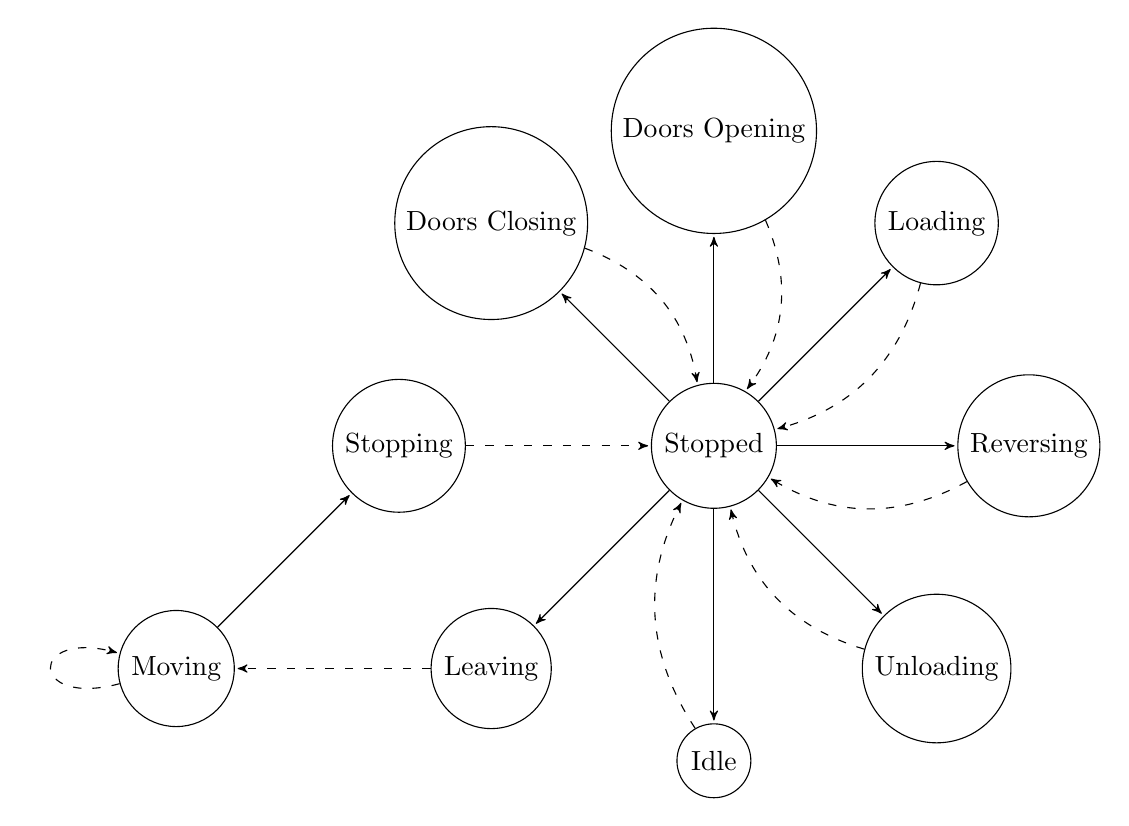
\begin{tikzpicture}[>=stealth',shorten >=1pt,auto,node distance=4cm]
		\node[state]	(stpd)						{Stopped};
  		\node[state] (drop)		[above of =stpd]		{Doors Opening};
  		\node[state] (load)		[above right of =stpd]	{Loading};
  		\node[state] (revs)		[right of =stpd]		{Reversing};
  		\node[state] (unld)		[below right of =stpd]	{Unloading};
  		\node[state] (idle)		[below of =stpd]		{Idle};
  		\node[state] (leav)		[below left of =stpd]	{Leaving};
  		\node[state] (movg)	[left of =leav]		{Moving};
  		\node[state] (stpg)		[left of =stpd]		{Stopping};
  		\node[state] (drcl)		[above left of =stpd]	{Doors Closing};
  		
  		\path[->]
  		(stpd)		edge	[]			node	{}	(drop)
  				edge	[]			node	{}	(load)
  				edge	[]			node	{}	(revs)
  				edge	[]			node	{}	(unld)
  				edge	[]			node	{}	(idle)
  				edge	[]			node	{}	(leav)
  				edge	[]			node	{}	(drcl)
		(movg)	edge	[]			node	{}	(stpg)
  		;
  		
  		\path[->, dash pattern = on 3pt off 4pt]
  		(drop)		edge	[bend left]		node	{}	(stpd)
  		(load)		edge	[bend left]		node	{}	(stpd)
  		(revs)		edge	[bend left]		node	{}	(stpd)
  		(unld)		edge	[bend left]		node	{}	(stpd)
  		(idle)		edge	[bend left]		node	{}	(stpd)
  		(leav)		edge	[]			node	{}	(movg)
  		(stpg)		edge	[]			node	{}	(stpd)
  		(drcl)		edge	[bend left]		node	{}	(stpd)
  		(movg)	edge	[loop left]		node	{}	(movg)
  		;
	\end{tikzpicture}
	\caption{A transition diagram of the car action element of a car state}
	\label{caractions}
\end{figure}

\autoref{caractions} demonstrates the relationship between the ten car action states.  In this diagram, solid transition edges denote immediate action changes, while dotted lines denote state changes that are made via the agenda.  For example, if the car is in the Stopped state, and determines that the next required action is to reverse, it will immediately change its state to Reversing.  Since there must then be a delay before the car can do anything else (specified by the user as, for example, 1 second), it will add an event on the agenda for 1 second later.  This agenda event will tell the car to go back into the Stopped state.  Then it might determine that the next required action is to load passengers, so it will immediately change into the Loading state.  It will then calculate the amount of time that loading will take (based on the number of passengers to load, and the user-specified loading time per passenger) and add an event onto the agenda for when the car should re-enter the Stopped state.  Putting future events onto the agenda allows the immediate control to return to the main control loop, which can (if appropriate) serve Passenger Hall Call events and/or events for other cars in the mean time.

\subsubsection{Movement Mathematics}

When the car is in one of the Leaving, Moving and Stopping action states, the car must work out the parameters of its next state.  If the current state is Leaving or Moving, then the next state will be a decision point for whether or not to stop at the next floor.  If the current state is Stopping, then the next state will be Stopped at the next floor.  In each case, we know all of the following information:

\begin{tabular}{l l}
	$U$ & The current speed (ms\textsuperscript{-1}) \\
	$F$ & The current floor \\
	$G$ & The next floor \\
	$S$ & The distance to the next floor (m) \\
	$A$ & The rate of acceleration of the car (ms\textsuperscript{-2}) \\
	$D$ & The rate of deceleration of the car (\textit{positive} ms\textsuperscript{-2}) \\
	$M$ & The maximum speed of the car (ms\textsuperscript{-1})
\end{tabular}

We are required to find the following parameters, which define our next state:

\begin{tabular}{l l}
	$V$ & The speed of the car when it reaches that state (ms\textsuperscript{-1}) \\
	$T$ & The time taken to reach the state (s)
\end{tabular}

In each case, we use the following basic equations of motion:

\begin{equation} \label{motioneq1} v=u+at\end{equation}
\begin{equation} \label{motioneq2} v^2=u^2+2as\end{equation}
\begin{equation} \label{motioneq3} s=ut+\frac{1}{2}at^2\end{equation}

In these equations, the variables are generically defined as follows:

\begin{tabular}{l l}
	$t$ & The duration of a time interval (s) \\
	$s$ & The distance travelled during the time interval (m) \\
	$u$ & The speed at the beginning of the time interval (ms\textsuperscript{-1}) \\
	$a$ & The rate of acceleration (ms\textsuperscript{-2}) \\
	$v$ & The speed at the end of the time interval (ms\textsuperscript{-1})
\end{tabular}

Once $V$ and $T$ have been found, the next car state will be placed on the agenda for $T$ seconds from now.

Here, I will demonstrate the maths for upward movement.  The maths for downward movement is analogous.

\paragraph{Moving state}

The Moving state applies when the car is moving, has reached a decision point, and has decided not to stop.  The parameters of the next decision point must be calculated, and there are two scenarios that must be considered.

The first, and simplest, scenario is where the car will accelerate until it reaches the decision point for the next floor, then decide whether or not to start slowing for the floor.  In this case, we simply need to find the point Q at which the acceleration curve from our current state crosses the deceleration curve for the next floor (\autoref{movingsimp}).

\begin{figure} [h]
	\centering
	\includegraphics{moving_simp.png}
	\caption{Simple case while moving}
	\label{movingsimp}
\end{figure}

We first find the distance from here to point $Q$, which we will call $Q_D$.  By two applications of \autoref{motioneq2} we find that:
\[Q_V^2=U^2+2AQ_D \text{ (for the acceleration curve)}\]
\[ \text{and } 0=Q_V^2-2D(S-Q_D) \text{ (for the deceleration curve).} \]

Note that $Q_V$ is the speed that we will have at point $Q$.  Combining these two equations we find that
\[ Q_D=\frac{2DS-U^2}{2(A+D)} \]

It is now trivial to find $V$ and $T$ as required, since
\[ V^2=Q_V^2=U^2+2AQ_D \text{ from \autoref{motioneq2}} \]
\[ \text{and } T=Q_T=\frac{Q_V-U}{A} \text{ from \autoref{motioneq1}. } \]

The second scenario is invoked when we find that $Q_V$ exceeds the maximum speed $M$ that our car can travel at.  In this case we will accelerate to some point $P$ on the acceleration curve (at which $P_V=M$), then move at a constant speed of $M$ until we reach the decision point $R$, the latest point at which we can decelerate to the next floor from speed $M$ (\autoref{movingcomp}).

\begin{figure} [h]
	\centering
	\includegraphics{moving_comp.png}
	\caption{Complex case while moving}
	\label{movingcomp}
\end{figure}

The parameters of the point $P$ on our acceleration curve are trivial to find:
\[ P_V=M \text{ by definition,} \]
\[ P_T=\frac{P_V-U}{A} \text{ from \autoref{motioneq1}} \]
\[ \text{and } P_D=UP_T+\frac{1}{2}AP_T^2 \text{ from \autoref{motioneq3}.} \]

Then, the distance from our initial point to point $R$, named $R_D$, can be found from the following equation
\[ 0=R_V^2-2D(S-R_D) \text{ from \autoref{motioneq2},} \]
which rearranges to give
\[ R_D = S - \frac{R_V^2}{2D} \text{.} \]

Then, since the movement from $P$ to $R$ is constant at speed $M$ the required values $V$ and $T$ can be calculated as
\[ T = R_T = P_T+\frac{R_D-P_D}{M} \]
\[ \text{and } V = R_V = M \text{.} \]

Note that the above logic and equations also hold for the common case where the current speed of the car is already at the maximum speed.  In such a scenario, it is correctly calculated that $P_T=P_D=0$.

\paragraph{Leaving state}

The Leaving state applies when the car is stopped and about to start leaving.  The parameters of the first decision point that will be encountered by the car must be calculated.  The logic and equations for the Leaving state are the same as those for the Moving state, but if the car is in the Leaving state then $U=0$.  \autoref{leavingsimp} and \autoref{leavingcomp} demonstrate these scenarios graphically.

\begin{figure} [h]
	\centering
	\includegraphics{leaving_simp.png}
	\caption{Simple case while leaving}
	\label{leavingsimp}
\end{figure}

\begin{figure} [h]
	\centering
	\includegraphics{leaving_comp.png}
	\caption{Complex case while leaving}
	\label{leavingcomp}
\end{figure}

\paragraph{Stopping state}

The Stopping state applies when the car is moving, has reached a decision point, and has decided to stop.  If the car is in the Stopping state, the maths is very simple.  The next state is reached by following the deceleration curve straight down to stopping at the floor.  Therefore,
\[ V=0 \text{ by definition of Stopping} \]
\[ \text{and } T=\frac{U}{D} \text{ from \autoref{motioneq1}.} \]

\subsection{Allocator Component}
\label{coresimallocatordescription}

The Allocator component in the Core Elevator Simulator consists of an Interface class, named IAllocator, defining the methods that an Allocator implemented by the user must include.  In fact, the IAllocator interface is very simple and contains just one method which is called by the main control loop when a new PassengerGroup arrival is taken from the agenda:

\lstset{language=[Sharp]C, basicstyle=\ttfamily\tiny, breaklines=true, breakatwhitespace=true }
\begin{lstlisting}
interface IAllocator
{
	/// <summary>
	/// Allocates a given group of passengers to a specific car within
	/// the given building, based on the relevant allocation method
	/// </summary>
	/// <param name="group">The PassengerGroup to be allocated</param>
	/// <param name="building">The Building holding the domain model</param>
	void AllocateCall(PassengerGroup group, Building building);
}
\end{lstlisting}

There is also an enum class, AllocatorType, which defines the names of all of the allocators.  Then, there is a static method which takes a specific AllocatorType enum value and returns an instance of the relevant Allocator as implemented by the user.

In order to demonstrate the ease with which a new Allocator can be added, I will include an example of a very simple allocation algorithm, the ClosestCar algorithm, which simply allocates each call to whichever car is closest to the call at the time the call is made, ignoring the directions in which cars are moving.

Firstly, the user must create a new class, which implements IAllocator.  As described, the AllocateCall method must be implemented, as follows:

\begin{lstlisting}
class ClosestCarAllocator : IAllocator
{
	/// <summary>
	/// Allocates a given group of passengers to a specific car within
	/// the given building, based on the ClosestCar allocation method
	/// </summary>
	/// <param name="group">The PassengerGroup to be allocated</param>
	/// <param name="building">The Building holding the domain model</param>
	public void AllocateCall(PassengerGroup group, Building building)
	{
		// compile list of all cars
		List<ICar> cars = new List<ICar>();
		building.Shafts.ForEach(s => s.Cars.ForEach(c => cars.Add(c)));
		// get closest car
		var car = cars.OrderBy(c => Math.Abs(c.State.Floor - group.Origin)).First();
		// allocate call
		car.allocateHallCall(new HallCall(group));
	
		// update the PassengerGroup data with the time at which
		// the hall call was made
		group.changeState(PassengerState.Waiting, Simulation.agenda.getCurrentSimTime());
	}
}
\end{lstlisting}

Secondly, the name of the Allocator must be added to the AllocatorType enum:

\begin{lstlisting}
enum AllocatorType
{
	Manual,
	Random,
	ClosestCar
}
\end{lstlisting}

Finally, the new Allocator must be added to the mapping method:

\begin{lstlisting}
public static IAllocator getAllocator(AllocatorType allocator)
{
	switch (allocator)
	{
		case AllocatorType.Manual:
			return new ManualAllocator.ManualAllocator();
		case AllocatorType.Random:
			return new RandomAllocator.RandomAllocator();
		case AllocatorType.ClosestCar:
			return new ClosestCarAllocator.ClosestCarAllocator();
	}
	
	return null;
}
\end{lstlisting}

Once the user has performed these three steps, the simulator can be recompiled and the new Allocator can be used.

\subsection{Passenger Distribution Generator}

The purpose of the Passenger Distribution generator is to load an XML `specification' file, which contains the parameters of the Poisson distributions for the various floors.  Based on this, it outputs a second XML file containing a list of specific passenger groups, with their arrival times, sizes, origins and destinations.  The arrival times of these passenger groups should follow the relevant Poisson distributions as taken from the specification file.  An example specification file is shown below.

\lstset{language=XML}
\begin{lstlisting}
<ArrivalFloors>
	<ArrivalFloor Floor="0">
		<DestinationFloor Floor="1" ArrivalsPerMinuteMean="5.0" GroupSizeMean="2" />
		<DestinationFloor Floor="2" ArrivalsPerMinuteMean="3.0" GroupSizeMean="2" />
	</ArrivalFloor>
	<ArrivalFloor Floor="1">
		<DestinationFloor Floor="0" ArrivalsPerMinuteMean="0.5" GroupSizeMean="1" />
		<DestinationFloor Floor="2" ArrivalsPerMinuteMean="1.0" GroupSizeMean="1" />
	</ArrivalFloor>
	<ArrivalFloor Floor="2">
		<DestinationFloor Floor="0" ArrivalsPerMinuteMean="0.3" GroupSizeMean="1" />
		<DestinationFloor Floor="1" ArrivalsPerMinuteMean="0.5" GroupSizeMean="1" />
	</ArrivalFloor>
</ArrivalFloors>
\end{lstlisting}

This example specification is for up-peak traffic between three floors.  The first <ArrivalFloor> element specifies the mean number of arrivals per minute at floor 0 as 5 groups going to floor 1, and 3 groups going to floor 2.  Similarly, the mean is 0.5 groups per minute going from floor 1 to 0, and 1 group per minute going from 1 to 2.  0.3 groups per minute go from floor 2 to 0, while 0.5 groups per minute go from 2 to 1.  You will also see that the sizes of groups boarding at floor 0 are generally larger, with an average of 2 people as opposed to an average of 1 person per group for other movements.

The passenger distribution generator was run with the above specification file, and configured to create a schedule for a period of 10 minutes, from 13:00:00 to 13:10:00.  An extract from the file is shown here, but the full schedule is available in the appendix.

\begin{lstlisting}
<PassengerGroups>
	<PassengerGroup ArrivalTime="03/03/2014 13:00:02" Size="1" Origin="0" Destination="2" />
	<PassengerGroup ArrivalTime="03/03/2014 13:00:11" Size="2" Origin="0" Destination="1" />
	<PassengerGroup ArrivalTime="03/03/2014 13:00:20" Size="1" Origin="1" Destination="2" />
	<PassengerGroup ArrivalTime="03/03/2014 13:00:28" Size="2" Origin="0" Destination="1" />
	<PassengerGroup ArrivalTime="03/03/2014 13:00:31" Size="2" Origin="0" Destination="1" />
	<PassengerGroup ArrivalTime="03/03/2014 13:00:34" Size="2" Origin="0" Destination="1" />
	<PassengerGroup ArrivalTime="03/03/2014 13:00:48" Size="2" Origin="1" Destination="2" />
	<PassengerGroup ArrivalTime="03/03/2014 13:00:50" Size="1" Origin="0" Destination="1" />
	<PassengerGroup ArrivalTime="03/03/2014 13:00:52" Size="3" Origin="0" Destination="2" />
	<PassengerGroup ArrivalTime="03/03/2014 13:00:59" Size="1" Origin="0" Destination="2" />
	<PassengerGroup ArrivalTime="03/03/2014 13:01:12" Size="1" Origin="2" Destination="1" />
	<PassengerGroup ArrivalTime="03/03/2014 13:01:15" Size="4" Origin="0" Destination="1" />
	<PassengerGroup ArrivalTime="03/03/2014 13:01:51" Size="2" Origin="0" Destination="1" />
	<PassengerGroup ArrivalTime="03/03/2014 13:01:52" Size="1" Origin="0" Destination="1" />
	<PassengerGroup ArrivalTime="03/03/2014 13:02:31" Size="3" Origin="0" Destination="2" />
	<PassengerGroup ArrivalTime="03/03/2014 13:02:54" Size="2" Origin="0" Destination="2" />
	.
	.
	.
</PassengerGroups>
\end{lstlisting}

The format of this file is fairly straightforward; each Passenger Group in the schedule is shown as a single element in the file, with attributes storing its time of arrival, size, origin and destination.  This file is loaded at the start of a simulation run and all of the Passenger Group arrivals are added to the agenda.

\subsubsection{Generating values with a Poisson distribution}

The schedule is generated by using Knuth's algorithm for Poisson distributions, which is described by the following pseudocode:  \citep{Ahrens1974, Atkinson1979}

\begin{lstlisting}
function PoissonDistributedRandomNumber(mean):
	L := e ^ (mean * -1)
	k := 0
	p := 1

	do while p > L:
		k := k + 1
		u := random[0, 1] // u is a random real number in the interval [0, 1]
		p := p * u

	return k - 1
\end{lstlisting}

When generating the schedule, we progress through time in steps specified by the user (in this example we will use 1 second time slices).  At each time step, we calculate the mean number of passenger groups for each movement in that time step (for a 1 second step, we divide the mean per minute by 60), and then use Knuth's algorithm to determine, based on that mean, how many arrivals we will have for each movement.  Then, for each arrival that we generate, we run Knuth's algorithm based on the mean group size for that movement to determine the size of the group.  The user specifies a maximum group size; if the size of a group is not between 1 and the user-specified maximum, we generate another value using Knuth's algorithm.

\subsection{Simulation Configuration}
All parameters of a simulation run are specified in a single configuration file, so that this configuration can be easily stored and re-run at a later date if desired.  A sample configuration file is shown in the appendix, but it includes the following parameters:
\begin{itemize}
	\item \textbf{Allocator} -- the name of the allocator that is to be used
	\item \textbf{Passenger Distribution parameters}
	\begin{itemize}
		\item Whether to load an existing distribution file or create a new one based on a given specification file
		\item Specification file path (if generating a new distribution)
		\item Maximum Passenger Group size (if generating a new distribution)
		\item Start time of distribution (if generating a new distribution)
		\item End time of distribution (if generating a new distribution)
		\item Resolution; the size of time steps (if generating a new distribution)
		\item Distribution file path
	\end{itemize}
	\item A selection of named sets of \textbf{Car Attributes}
	\begin{itemize}
		\item Maximum capacity
		\item Maximum speed
		\item Acceleration
		\item Deceleration
		\item DoorsOpenTime -- time taken to open doors
		\item DoorsCloseTime -- time taken to close doors
		\item DirectionChangeTime -- time taken to reverse
		\item PassengerBoardTime
		\item PassengerAlightTime
	\end{itemize}
	\item The domain model \textbf{Building}, with its lowest and highest floors, and the distance between floors specified.
	\begin{itemize}
		\item A selection of \textbf{Shafts}, within which
		\begin{itemize}
			\item A selection of \textbf{Cars}, each of which is linked to a set of Car Attributes as defined above, and a CarType (always Single-decker in the Core Elevator Simulator) as well as the floor at which the car is to be initialised.
		\end{itemize}
	\end{itemize}
	\item The path to a \textbf{Log File} -- the user can specify `auto' here, in which case an automatic file name will be generated based on the current date and time.
\end{itemize}

\section{Validation}

\textit{All validation work was performed independently of Craig, as were the code corrections made in response.}

The architecture of the Core Elevator Simulator allows each component to be validated separately, with only minimal verification on the ways in which they interact.

\subsection{Domain Model Component}

The most significant component to validate is the Domain Model component.  In order to test it I designed a specific passenger arrival schedule, containing a total of 13 groups and 39 passengers arriving over the course of 2\textonehalf minutes, that would result in each workflow within the Car domain logic being tested.  Bearing in mind the architecture of the simulator, a couple of simplifications were made, which will be briefly tested later:  Firstly, the test modelled a building with just 3 floors, since this was enough to give confidence about the performance over a larger number without increasing the complexity of the hand-calculations.  Secondly, since the cars do not interact with each other in the Core Elevator Simulator, I built a dummy allocator that would assign all calls to car 0, meaning that all calls would be handled by the same car.

Using Microsoft Excel to maintain a trace table, I worked through the way in which the car should behave as the different calls came in, performing all of the movement calculations and other mathematics by hand.  I calculated that the simulation run with my designed passenger arrival schedule would take 4 minutes and 14 seconds, and noted down the specific boarding and alighting times of each Passenger Group.  I also had a record of every state change that would take place in the car during the simulation run, which is shown in the appendix.

The test run included two scenarios where the car could not serve the calls due to lack of capacity, and it handled this correctly.  It also included cases where hall calls came in as the doors were closing.  The expected behaviour was for the car to reopen the doors and serve the hall calls before leaving.

There were times when the car would set off from floor 2, heading to floor 0 and then a hall call would come in at floor 1 just after it had left.  In this case, the expected behaviour was for the car to make an unexpected stop at floor 1, as long as the call came in before the car had passed the final decision point for floor 1.

Initially, when I ran the simulator for the first time on the specific passenger arrival schedule I was encouraged to see that for the first 45 seconds, the logs showed that the car was behaving exactly as I had predicted that it should in the trace table.  Unfortunately, after that the timings became about half a second out, which was the indicator of some flawed logic either in the simulator itself or in my hand-calculated trace table.  Having seen that the discrepancy came on the first occasion that the car was directed to pass a floor without stopping, I placed a breakpoint in that logic to find out if there was any problem.

In fact, there was a problem.  I had erroneously implemented the formula for finding PD as follows
\[ P_D = U + \frac{1}{2}AP_T^2 \text{,} \]
when, in fact, the correct formula is slightly different, as follows
\[ P_D = UP_T + \frac{1}{2}AP_T^2 \text{.} \]

After I had corrected this implementation, I tried the simulation run again and this time found that everything was behaving as expected.  All of the car state changes happened at the right time (within the 10-millisecond accuracy to which I had done my hand calculations), and all of the passenger boarding and arrival times were as expected too.  I am now confident that the Domain Model component of the Core Elevator Simulator behaves correctly.

In order to test the first of the two assumptions mentioned above, I reperformed the test using a shaft with 11 floors.  I modified the passenger arrival schedule described above so that passengers' origin and destination floors were all multiplied by 5, such that they all took place at floor 0, 5 or 10.  I then divided the interfloor distance by 5, so that the distances between each of the `used' floors was the same as before and the same maths calculations for broad movement could be used.  The time taken by the simulation was the same, and the result criteria were identical.  This demonstrated that the addition of extra floors between the `used' floors did not cause any problem, even though the car now had to go through many more state changes (at different speeds and locations) as it passed the decision points for each floor.

To test the second assumption, I took the original passenger arrival schedule and made two copies of it.  I offset all of the arrival times by 5 minutes in the first copy, and by 10 minutes in the second.  I then merged the three schedules into 1, which was obviously three times as large as the original.  I wrote a simple Allocator which allocated the first instance of each passenger group to Car 0, the second (5 minutes later) to Car 1, and the third (10 minutes later) to Car 2.  This was possible by maintaining a record in the Allocator of calls that had been served by each car and cross-matching new calls with previously-served calls.  The expected behaviour was that the mean results would be the same as they were in the original test, since the cars effectively performed the same test in parallel with 5 minutes separation to the start time.  The actual behaviour was as expected, giving me confidence that the cars in separate shafts do indeed behave independently of each other without any fault.

\subsection{Allocator Component}

Since the Allocator component will be re-implemented for each allocation algorithm that is run on the simulator, it doesn't really make sense to completely validate it at this stage.  However, in order to test the general interactions between the Allocator and the Domain Model component I have used the basic ClosestCar allocator as described above.  I then used a Manual allocator, which asks the user to allocate calls to cars, to make the decisions in my head (in the way that I believe the ClosestCar allocator should allocate them) and ensure that the behaviour of the simulator when using the ClosestCar allocator matches the behaviour when I make the decisions myself.

After running the simulation in both scenarios (with the same passenger arrival schedule as used in the domain model component tests), I found that the logs were identical.  Therefore, I am confident that the allocator component is behaving as it should.  It would not be useful to print the entire log here, but I will print the evaluation results which can be used for later verification if necessary:

\begin{lstlisting}
Average waiting time:                4.92269230769231
Average squared waiting time:        126.226432384615
Average time to destination:         22.3131538461538
Average squared time to destination: 782.275027153846
Longest waiting time:                38.249
Longest time to destination:         66.667
\end{lstlisting}

When the simulator is used with new allocation algorithms, care should be taken to ensure that the new Allocators have been implemented correctly, and tests should be performed to validate the implementations.

\chapter{TCOS Elevator Simulator}
\label{teschapter}

\section{Introduction}

This chapter describes the portion of the project during which I extended the Core Elevator Simulator to work for the Two Cars in One Shaft (TCOS) case.

\section{Additional Requirements}

\subsection{Specification of Requirements}

The following is a list of additional requirements that had to be met by the TCOS Elevator Simulator.  All of the requirements for the Core Elevator Simulator still applied, but will not be listed again here.  The only exception was that the requirement to be able to simulate systems \textit{without} Destination Control no longer applied, since TCOS systems always use Destination Control.

\subsubsection{Functional Requirements}

	\begin{enumerate}
		\item To be able to simulate the use, and evaluate the performance, of algorithms designed for the allocation of calls to cars in TCOS elevator systems.  The evaluation objectives must include those specified in the requirements for the Core Elevator Simulator.
		\item It should be possible to use, in one simulation, traditional elevator shafts (with exactly one car) and TCOS elevator shafts.
		\item In TCOS shafts, there should be a `garage' floor below the ground floor, in which the lower car can park, leaving the upper car with access to all passenger floors.
		\item Cars should have an optional `parking' behaviour so that when they become Idle they move to wait at a specific floor rather than just waiting in their current location.
		\item In TCOS shafts, the lower car should not accept call allocations which include the highest floor.  There is no restriction on which calls the upper car can accept.
	\end{enumerate}

\subsubsection{Non-Functional Requirements}

	\begin{enumerate}
	\setcounter{enumi}{5}
		\item The TCOS extension should avoid changes to the existing code that are so significant as to prevent re-integration with the Core Elevator Simulator line.  This will allow the TCOS simulator to be combined with other extensions made in parallel, making a single general purpose simulator.
		\item The TCOS extension should be built in such a way that it can be further extended to handle Many Cars in One Shaft (MCOS) cases (i.e. cases where a single shaft might contain 3 or more cars).
	\end{enumerate}

\subsection{Justification of Requirements}

The above requirements are justified as follows.

Requirement 1 specifies that the same evaluation objectives should be used in the TCOS Elevator Simulator as in the Core Elevator Simulator.  The reason for this is that it allows direct comparisons to be made between the performance of elevator groups containing TCOS shafts and those only containing traditional shafts.  With these comparisons available, inferences could be made about the scenarios in which TCOS systems can provide better performance than traditional systems.

In some scenarios, a building operator might choose to upgrade some subset of their elevator shafts to TCOS, while leaving the remaining shafts operating in the traditional manner.  Requirement 2 allows different such scenarios to be evaluated.

The garage floor in requirement 3 allows the lower car in a TCOS shaft to park out of the way, so that the upper car can visit all floors.  The parking functionality in requirement 4 allows the Allocator to make use of this floor, as well as having the upper car automatically park at the top floor so as to maximise the floors available to the lower car.

Requirement 5 stops the deadlock situation whereby a call for the top floor is allocated to the lower car, which can never reach the call due to the presence of the upper car.

Requirements 6 and 7 are included to ensure that the TCOS Elevator Simulator can be put to best use by me and others following the end of this project.

\section{Domain Assumptions}

There are a number of assumptions made about the TCOS case in addition those made for the Core Elevator Simulator.
	\begin{enumerate}
		\item The separation of cars within a shaft is controlled by ensuring that no two cars may occupy the same floor at the same time.
		\item When a car is moving from one floor ($a$) to the next ($b$), it is considered to occupy both floors at the same time.  Therefore the other car may not start moving towards floor $a$ until the car has reached floor $b$.
		\item No further separation is enforced between cars except as specified and implied by the assumptions above.
		\item No car will stop between floors.
	\end{enumerate}

\section{High Level Design Decisions}

The TCOS case introduced some complications to the constraints, which mean that decisions had to be made about the control logic in the Domain Model component.  Various strategies were considered in order to avoid deadlock or collision between cars.

\subsection{Option 1: Dynamic `Zoning' Approach}

This approach works by considering each car within a shaft to have an exclusive zone of floors transiently defined as the minimal set of consecutive floors containing (a) the current floor of the car, (b) the car's park floor, and (c) the locations of all calls currently assigned to the car.  When the Allocator attempts to assign a call to a car, the car must either accept or reject the call based on the following rules:
	\begin{enumerate}
		\item If both the origin and destination of the call are within the car's current zone, the call will be accepted.
		\item Otherwise, if both the origin and destination lie within the range of floors that the car's current zone can be extended into without overlapping with the zone of another car in the same shaft, the call will be accepted and the car's current zone will be extended accordingly.
		\item Otherwise, the call will be rejected and the Allocator will have to allocate the call to another car.
	\end{enumerate}

In this case, the park floors should be fixed as the highest floor (for the upper car) and the garage floor (for the lower car).

This approach very effectively separates the cars and does so without ultimately limiting the range of floors that any car can serve (for example, with appropriate Allocator behaviour, the upper car could conceivably serve a call at the ground floor, if the lower car is parked at the garage floor).  However, it is inefficient in that it could restrict the allocation of calls that might actually be feasible.  For example, if the upper car is at floor 8, and the lower car is travelling down from floor 4 to floor 1, it might be reasonable to allocate a call at floor 3 to the upper car.  This approach would not allow the allocation.

\subsection{Option 2: Conflict Resolution Approach}

This more complicated approach allows any call to be allocated to any car at any time, and then relies on the control logic to resolve conflicts between cars.  In general, there are two types of conflict: one where the cars are travelling in the same direction but the car in front is delaying the car behind and the other where the cars are both travelling towards each other.  The former of these is simple to resolve from a conceptual perspective – the one behind must wait for the other to move out of the way before proceeding.  The latter presents some issue as one car (a `slave') must reverse for some distance to allow the other one (the `master') to serve its calls.  Some method of determining which car would be given priority would be required in order to use this approach.

While this approach has the potential to solve the efficiency problem of option 1, it also has some problems of its own.  For example, the master-slave behaviour would result in some conflict with the passenger expectation constraints (i.e. that a car must not change direction if it currently has passengers on board).  Additionally, it means that some non-trivial logic which is conceptually part of the allocation process is fixed within the Domain Model component.

\subsection{Option 3: Overlapping Dynamic Zoning Approach}

The third option is similar to option 1, but it allows the zones of the two cars to overlap as long as the zone of the upper car does not contain the current floor of the lower car and vice-versa.  In this case, the set of floors that are in the zones of both cars is known as the overlap zone.  Only one of the cars may enter the overlap zone at a time, and this permission is granted to whichever one gets there first.  For example, if the overlap zone is floors 4, 5 and 6, and the lower car attempts to visit floor 4 while the upper car is still at floor 8, the lower car will continue to floor 4 and subsequently floors 5 and 6.  In the meantime, the upper car will be held at floor 7.  When the lower car leaves floor 6 to return to floor 5 the overlap zone will now only contain floors 4 and 5, so the upper car will be allowed to proceed to floor 6, and so on.

The following rules would be used to decide whether or not to accept a hall call:
\begin{enumerate}
	\item If both the origin and destination of the call are within the car's current zone, the call will be accepted.
	\item Otherwise, if the car's current zone contains a floor already occupied by the other car in the shaft, and both the origin and destination of the call are within the other car's zone without being the last floor in its zone, the call will be accepted and the car's current zone will be extended accordingly.
	\item Otherwise, if both the origin and destination lie within the range of floors that the car's current zone can be extended into without including the current floor of the other car in the same shaft, the call will be accepted and the car's current zone will be extended accordingly.
	\item Otherwise, the call will be rejected and the Allocator will have to allocate the call to another car.
\end{enumerate}

Note that if one car has already entered the overlap zone, the second rule allows the waiting car's zone to expand further past the other car.  This does not cause any problem, so long as the other car's zone always protrudes at least one floor further so as to avoid deadlock occurring later on.

As with option 1, the park floors for the upper and lower cars should be the highest floor and the garage floor respectively.

Option 3 is more efficient than option 1 in that it allows some feasible call allocations that option 1 does not allow.  However, it manages to extend the possibilities without contravening the passenger expectation constraints or the conceptual logic architecture of the simulator.

\subsection{Option 4: Extended Overlapping Dynamic Zoning Approach}

The fourth option considers that a car's zone is the minimal set of floors that contains (a) the current floor of the car, (b) the car's park floor, and (c) all floors that the car will visit before its next reversal.  This is different from the zones defined in options 3 and 4 as it only includes the calls in P1 and, if it is beyond the furthest location of all P1 calls, the first call in P2.

This option extends option 3 to allow one car's zone to `absorb' the current floor of the other car, provided that the other car's zone does not already include this car's current floor (i.e. this car is not inside the overlap zone).  The result of this absorption is that the other car is now inside the overlap zone, and thus this car must wait for the other car to leave before it can enter.

The changes to the zone definition mean that if a car is travelling towards its park floor, none of the floors behind it are included in its zone, meaning that the other car can follow it if it wants to without ending up in the situation where both cars are in the overlap zone.  However, in order to avoid a deadlock situation, if the car is travelling towards its park floor it must continue to do so until it has left the zone of the other car before reversing, so as to allow the other car to attend its calls.

In this option, the rules for accepting and rejecting calls are as follows:
	\begin{enumerate}
		\item If the call is a P3 call, the call will be accepted.
		\item Otherwise, if both the origin and destination of the call are within the car's current zone, the call will be accepted.
		\item Otherwise, if the car's current floor is not inside the overlap zone, and both the origin and destination of the call are within the other car's zone without being the last floor in its zone, the call will be accepted and the car's current zone will be extended accordingly.
		\item Otherwise, if the car's current floor is inside the overlap zone, and both the origin and destination lie within the range of floors that the car's current zone can be extended into without including the current floor of the other car in the same shaft, the call will be accepted and the car's current zone will be extended accordingly.
		\item Otherwise, the call will be rejected and the Allocator will have to allocate the call to another car.
	\end{enumerate}

Note that the lower car can never accept a call that requires it to visit the highest floor, and the upper car can never accept a call that requires it to visit the garage floor.  This rule is implicitly satisfied by the rules given above (a car cannot accept a call where either the origin or destination floor is the last floor in the other car's zone).

Again, the park floors for the upper and lower cars should be the highest floor and the garage floor respectively.

This option further builds on the benefits of options 1 and 3, without contravening either the passenger expectation constraints or the conceptual logic architecture of the simulator.  For this reason, I chose to use option 4 in the TCOS Elevator Simulator.

\section{Detailed Description of Changes Made}

In this section I will describe the changes that were necessary in order to extend the Core Elevator Simulator for the TCOS case.  The majority of the changes were to the Domain Model component, though minor changes were also necessary in the Allocator and Simulation Configuration components.

\subsection{Domain Model Component}

There was a large amount of logic that needed to be added to the Domain Model in the TCOS Elevator Simulator.  In order to maintain the generality of the simulator (so that it could still be used for simulations including traditional elevator shafts as well as TCOS shafts) a new TCOSCar class was added, and the traditional Car class was left largely unchanged.  The Core Elevator Simulator had been designed such that the traditional Car class implemented an interface, ICar, and all interactions with the Car were via the ICar interface.  This meant that the TCOSCar class simply needed to interface the ICar interface in order to be compatible with the rest of the program.

Since the Extended Overlapping Zoning Approach (option 4, discussed above) requires that a TCOS car can reject call allocations, it was necessary to modify the ICar interface slightly so that the allocateHallCall method, called by Allocators to allocate a call to a car, returned a Boolean value indicating the success (true) or failure (false) of the allocation.  The traditional Car class had to be modified accordingly, simply returning true (for success) in all cases.

Aside from the minor `housekeeping' changes described above, the following three methods were added in the TCOS implementation, corresponding to certain aspects of logic in option 4:
	\begin{description}
		\item[CanAcceptHallCall] Based on the rules described in option 4, this method works out whether or not a call can be accepted at the current time, based on the circumstances of both cars in the shaft and the calls currently allocated to them.
		\item[CanMoveToNextFloor] This method works out whether or not the car is permitted to move forward to the next floor.  This is necessary because a car cannot enter the overlap zone while the other car is within it.
		\item[MustContinueInCurrentDirection] This method works out whether or not the car must continue forward in order to allow the other car to visit its calls, even if this car needs to reverse before it can serve its own calls.  As described in option 4, if the car is in the overlap zone and travelling back towards its park floor it must continue forward until it has left the overlap zone, so as to avoid causing a deadlock situation.
	\end{description}
	
All of these three methods require knowledge of the current zones applicable to the two cars in the shaft.  Therefore, a CurrentZone property was added in the TCOSCar class, which calculates and returns a list of all floors in the current zone according the definition described in option 4.  Additionally, a CurrentFloorsOccupied property was added in the TCOSCar class, which returns a list of up to 2 floors that the car is currently occupying.  If a car is stopped at floor 4, this list only contains the value 4, while if it is moving from floor 4 to floor 5, the list contains both 4 and 5 until it arrives at floor 5 when it will contain just 5.

A new action was added to the CarAction options, named `Waiting', which a TCOS car uses when it is stationary waiting for the other car to perform tasks before it can move.  When one car in the shaft moves, it notifies the other car so that the other car can, if appropriate, re-assess the situation and decide whether or not to continue waiting.  The waiting car will begin moving again once the other car has started moving back towards its park floor.

It was also necessary to change the behaviour of the cars so that, instead of simply stopping in situ and changing its action to Idle when there are no calls to serve, the car would move to its designated park floor at this stage before entering changing to a new action, named `Parked'.

\subsection{Allocator Component}

The only change necessary in the Allocator component related to the fact that a car can now reject hall call allocations, with the allocation method returning true or false to indicate whether or not the allocation was accepted.  Therefore, Allocators must be aware of the potential for an allocation to fail and, if appropriate, implement code to handle an allocation failure and attempt allocation to another car.

\subsection{Simulation Configuration}

The first change necessary in the Simulation Configuration component was to allow simulation configuration files to specify the park floor of each car.  This was implemented by adding a `parkFloor' attribute to the `Car' tag in the XML config files, the value of which is passed to the corresponding car at the start of the simulation.

The second change was to add `TCOS' as an option for the car type, so that the user could select to use TCOS cars in the simulation.

\section{Validation}

\subsection{Domain Model Component}
As with the Core Elevator Simulator, the most significant validation required in the TCOS Elevator Simulator is in the Domain Model component.  Again, since each car only interacts with the other car in its shaft, it was appropriate to focus the testing on the behaviour of cars within a single shaft.  This time, I used a building consisting of 10 floors, numbered 0 to 9, as well as a garage floor below floor 0 (numbered -1) which could not be used by passengers.  The passenger arrival schedule contained 9 passenger groups, totalling 39 people, arriving over the course of 2\textonehalf minutes.  I built an allocator named TwoZonesAllocator which would allocate each hall call to either the upper or lower car depending on the origin and destination floors of the passenger group involved (if the average of the origin and destination was greater than or equal to 4.5 the allocator would first attempt to allocate it to the upper car, otherwise it would first attempt to allocate it to the lower car).  If the first allocation attempt failed, it would allocate it to the other car instead.

Again, I used Microsoft Excel to maintain a trace table of the behaviour of both cars in the shaft, performing all calculations by hand.  I calculated that the full simulation run would take a total of 4 minutes and 54 seconds, and kept a record of the boarding and alighting times of each passenger group.  The full trace table, including every state change that took place, is shown in the appendix.

The passenger arrival schedule was designed to invoke all of the code path scenarios available, specifically testing the following cases:
	\begin{itemize}
		\item A car stops to pick up passengers that cannot be accommodated due to lack of available space.  In this scenario the car was to revisit and attempt to pick up the passengers later on, and it was important that the zoning approach could handle this change of circumstances appropriately.
		\item A car is closing its doors when it receives a new call to be served from this floor in this direction.  The car was to reopen its doors and allow the new passengers on.
		\item A car receives a call requiring it to stop at the next floor, while it is currently moving towards that floor.  Provided there is still time to stop, the car is to make an unexpected stop to pick up the passengers.
		\item A car wishes to enter the overlap zone when the other car already occupies the zone.  The car must wait for the other car to turn back before it can continue.
		\item A car has finished serving all calls in P1 and needs to reverse in order to serve P2 calls.  However, the other car has entered the overlap zone and needs to come to the floor that this car currently occupies.  This car must first continue away from its calls so that the other car can serve its calls, so as to avoid a deadlock scenario.
		\item A car has finished serving all calls in P1, P2 and P3.  It must return to its park floor and wait for further calls to be allocated.
		\item A car is inside the overlap zone when the allocator attempts to allocate a P1 call that would require the car to visit the floor at which the other car is currently waiting.  Since this would result in a deadlock scenario, the car must reject the call.
	\end{itemize}

When I first ran the TCOS Elevator Simulator configured as described above, the two cars in the shaft entered a deadlock scenario.  This meant that either there was a problem with the logic decided upon in option 4 (extended overlapping dynamic zoning) or that it had been incorrectly implemented in the code.  I placed a breakpoint in the code to be activated just before the deadlock scenario occurred so that I could examine the implementation and determine the cause of the problem.  It turned out that the implementation of the logic in the MustContinueInCurrentDirection method was flawed in that it only considered the floor of the other car's state, even if the other car had been authorised to proceed to the next floor and was moving towards it.  I changed the code to use the CurrentFloorsOccupied property of TCOSCar which includes the floor towards which a car has started moving.

After I had corrected this aspect of the code, I ran the simulation again and found that everything behaved as expected.  The car state changes happened at the right times (within the 10-millisecond accuracy to which I had performed my calculations), and all passenger boarding and arrival times were as expected, as well as the success and failure of call allocations.  I am now confident that my changes to the Domain Model in the TCOS Elevator Simulator are valid.  \autoref{tcosvalidationgraph} is an Excel-generated graph which shows the movement of the upper (pink) and lower (blue) cars with time, demonstrating the minimum distance maintained between the two cars.

\begin{figure} [h]
	\centering
	\includegraphics[width=\linewidth,keepaspectratio]{tcos_validation_movement_graph.png}
	\caption{The movement of the two cars during the validating simulation run}
	\label{tcosvalidationgraph}
\end{figure}

\subsection{Allocator Component}
The only change to the Allocator component was for Allocators to handle call allocation failures from Cars.  This was implicitly tested during the Domain Model tests described above and performed correctly.  However, it is still necessary that each new Allocator that is implemented should be properly validated as discussed in the Core Elevator Simulator part.

\part{Algorithms for TCOS Elevator Systems}

\chapter{Discussion of Allocation Algorithms}
\label{algdiscussion}

In this chapter, I will discuss a number of allocation algorithms that I have developed or adapted for use in the TCOS case.  In \autoref{algsimulation} and \autoref{algevaluation} I will describe the process of evaluating each of these algorithms on the TCOS Elevator Simulator, and discuss their performances.

\section{Estimated Time of Arrival Allocation (ETA)}
\label{algETAdescription}

The Estimated Time of Arrival (ETA) algorithm is an existing algorithm for traditional elevator systems which has been widely studied in the literature \citep{Rong2003, Nikovski2003} and performed well in simulations \citep{Rong2003}.  The algorithm happens to work in such a way that its concepts can be adapted for use in the TCOS case.  After briefly describing ETA in its original form, I will discuss three ways in which I have adapted it for TCOS systems.

ETA is an immediate allocation algorithm that aims to minimise the average waiting time of all passengers in the system.  Every time a new hall call is made, it considers allocating the call to each one of the cars in the system and estimates the cost each of the possible allocations.  It then allocates the call to the car which results in the lowest estimated cost.  The cost estimation function of allocating the call to a given car is made up of two parts: the estimated time taken for the car to reach the new call (Estimated Waiting Time), and the total additional waiting time caused to the other passengers currently waiting for the car (System Degradation Factor) \citep{Rong2003}.  The Estimated Waiting Time and System Degradation Factor are summed together to provide the total estimated cost.

A simple modification to ETA allows allocation costs to be estimated based on squared waiting times, thus preferring a narrower spread of results over one where some individuals benefit highly and others are severely disadvantaged.

\citet{Rong2003} present a reallocation variant of ETA, which allows calls to be retrospectively reassigned after the initial assignment, but since this is not compatible with Destination Control systems I will not describe it here.  They also describe methods of predicting passenger destinations in systems without Destination Control, but since Destination Control gives us full knowledge of the intentions of passengers as soon as they have made hall calls there is no need for us to consider these methods.

\subsection{Na\"{i}ve ETA}

The simplest method of adapting ETA for TCOS systems is simply to apply the basic cost estimation function to each car in the system ignoring the interactions between two cars in the same shaft.  The method of calculating the approximate cost is as follows:

Assume the following given time parameters (all in seconds):\\*
\begin{tabularx}{\linewidth}{l X}
	$Start$		& The time taken for a car to start moving from loading (including closing doors, additional time required for acceleration, etc.) \\
	$Stop$		& The time taken for a car to stop moving and start loading (including opening doors, additional time required for deceleration, etc.) \\
	$Travel$	& The time taken for a car to travel between floors once moving \\
	$Reverse$	& The additional time taken for a car to reconfigure its direction when stopped \\
	$Unload$	& The time taken for a single passenger to alight the car \\
	$Load$		& The time taken for a single passenger to board the car
\end{tabularx}

Using these time parameters, and the full knowledge of all passengers currently waiting for or travelling inside the car, predict, for each passenger group, the amount of time that they will have to wait before the car arrives to pick them up.  Then, consider allocating the new hall call to the car and the effect that this will have on the waiting times of the other passengers.  This effect is the System Degradation Factor (SDF) and can be stated as follows:
\[ SDF(c, h) = \sum\limits_{g \in G(c)} (EWT(g, c, G(c) \cup \left\{ h \right\}) - EWT(g, c, G(c)))\]
where $c$ is the car, $h$ is the new hall call to be allocated, $G(c)$ is the set of groups already allocated to car $c$ and $EWT(g,c,G(c))$ is the estimated time taken for car $c$ to reach call $g$ given the calls in $G(c)$ (estimated waiting time for $g$).

The total estimated cost of allocating call $h$ to car $c$ is as follows:
\[ Cost(c, h) = SDF(c, h) + EWT(h, c, G(c) \cup \left\{ h \right\}) \]

The cars are all ranked by their respective values of the estimated cost function.  If the most preferred car rejects the allocation (see the notes on option 4 in \autoref{teschapter} for why this might happen) then the second most preferred car will be attempted, and so on.

Estimated waiting times can be calculated en masse by doing a rough simulation of the behaviour of the elevator using the six time parameters above and noting the boarding times of each group.  It would be possible to perform this simulation more exactly by using the simulation methods employed by my own TCOS Elevator Simulator but this is computationally expensive and in real world applications allocation decisions must be quickly computable both to make the process more efficient from a customer perspective and to avoid the state of the system changing significantly during the course of the computation.  I consider that the small loss of accuracy from using an approximate method is unlikely to significantly affect the performance of the allocation algorithm, and the consequences of an occasional sub-optimal allocation are of less concern than the alternative risks.

\subsection{Conflict-sensitive ETA}
\label{algETAconflict}

An obvious flaw with the na\"{i}ve algorithm is that is does not account for the delay caused by two cars in the same shaft having conflicting movements.  In order to resolve this, I have designed a simple method of predicting the cost caused by conflicts.  Again, I have chosen this method so as to minimize the computational cost for the same reasons as discussed with the na\"{i}ve algorithm.  The general method is the same as described above, but the EWT must now take into account the behaviour of both cars, and their interactions, and the SDF must take into account the delay caused to passengers in the other car ($d$) as well as those in the allocation car ($c$).

In order to calculate the estimated waiting times of all groups in $G(c)$ and $G(d)$ we firstly work out an overlap region which is the range of floors that both $c$ and $d$ must visit in order to serve their respective calls.  We perform separate rough simulations of the behaviour of $c$ and $d$ as described for the na\"{i}ve algorithm but we take note of the times at which the car enters the overlap region and when it turns around to leave the region again (at which point the region becomes available to the other car).  If there is no overlap region (i.e. the calls in $G(c)$ and $G(d)$ relate to disjoint sets of floors) then no entries or reversals are recorded.  After completing the simulations we retrospectively analyse the times spent in the overlap region.  When two cars attempt to use the overlap region at the same time, it is assumed that the first car to arrive gets priority and that the second car must wait until the first has turned around before entering.  Therefore, the delay caused to the second car by waiting (easily calculated by taking the second car's entry time from the first car's reversal time) is added to all of its subsequent times.  As with the na\"{i}ve algorithm, we must calculate these estimated waiting times twice -- once including and once excluding the new hall call allocation -- in order to determine the SDF.

This method makes many assumptions about the behaviour of the cars, and in some cases has the potential to provide quite bad estimations (a small error in calculating times could have a significant propagation effect if it means that the order in which two cars approach the overlap region is predicted incorrectly) but it is expected to add value to the ETA method nonetheless.

\subsection{Load-sensitive ETA}

Another factor that can be considered in ETA allocation algorithms is the question of what happens if an allocation results in the capacity of the car being exceeded at some point.  As discussed previously, I have a simplification assumption that, should a passenger group be allocated to a car that cannot accommodate it when the car arrives, the passenger group will wait for the same car to go away and come back.  Since this is likely to come with great time costs for affected passenger groups, it is imperative that allocation algorithms do not result in over-allocation where possible.  I have therefore designed a variant of ETA whereby a high penalty cost is applied every time a passenger group cannot be accommodated by the car to which they have been allocated.  The penalty cost is a parameter that should be set equivalent to a very high number of seconds, so as to discourage these allocations.  It should be noted that an allocation might cause a later group not to be accommodated, even if the passenger group under allocation can be accommodated itself.  If an allocation results in 2 passenger groups being affected in this way, then the penalty cost will be applied twice, and so on for greater numbers.  The SDF is altered accordingly.  Assuming a high penalty cost value is chosen, this method has the effect of prioritising firstly the allocation that results in the fewest capacity-related problems, and resolving `ties' by minimising the original EWT costs described previously.

\section{Estimated Time to Destination Allocation (ETD)}
\label{algETDdescription}

The ETD algorithm is very similar to ETA, but with the difference that it attempts to minimise the average \textit{system} time (or squared system time) rather than the waiting time.  Usage of ETD in traditional elevator systems is hampered (to a greater extent than ETA) by the lack of information about passenger group destinations until they have boarded the car and pressed a button.  I expect that since the system with which we are concerned includes Destination Control we can make very effective use of this method without needing to speculate about passenger destinations.

The comments made about ETA in \autoref{algETAdescription} also apply to ETD, as do the variant adaptation methods described (na\"{i}ve, conflict-sensitive and load-sensitive).  I will briefly discuss the way in which these adaptations can be analogously applied to ETD.

\subsection{Na\"{i}ve ETD}

The six parameters described previously all still apply for ETD: $Start$, $Stop$, $Travel$, $Reverse$, $Unload$, $Load$.  The SDF and Cost methods are adapted as follows:

\[ SDF(c, h) = \sum\limits_{g \in G(c)} (EST(g, c, G(c) \cup \left\{ h \right\}) - EST(g, c, G(c)))\]
\[ Cost(c, h) = SDF(c, h) + EST(h, c, G(c) \cup \left\{ h \right\}) \]
where $c$, $g$, $h$ and $G(c)$ are equivalent to the same variables in ETA and $EST(g,c,G(c))$ is a method calculates the expected system time (from pressing the call button to exiting a car at the destination floor) of passenger group $g$ travelling in car $c$ with calls $G(c)$.

The rough simulation is performed in the same manner as with na\"{i}ve ETA.

\subsection{Conflict-sensitive ETD}

Conflict-sensitive ETD is completely analogous to Conflict-sensitive ETA.

\subsection{Load-sensitive ETD}

Again, Load-sensitive ETD is analogous to Load-sensitive ETA, but note that the penalty costs continue to be applied based on capacity at the time of loading rather than the time of alighting.  For the sake of a rough EST estimation, passenger groups are taken to travel in the car at the first `opportunity' irrespective of current load.  The penalty is partially intended to account for the amount of additional time that the group will have to wait for the car to serve other calls and then return and pick them up the next time.

\section{Minimal Overlapping Allocation (MOA)}

I have developed this simple allocation policy which attempts to minimise the amount of time lost by one car having to wait for the other car.  It does this by attempting to minimise the sizes of the overlap regions (as described in \autoref{algETAconflict}) throughout the system.  In this algorithm, the cost of allocating to a car $c$ which shares a shaft with car $d$ is the size of the extension caused to the existing overlap region between $c$ and $d$ (if any).  That is:

\[ Cost(c, d, h) = Overlap(c, d, G(c) \cup \left\{ h \right\}, G(d)) - Overlap(c, d, G(c), G(d)) \]

where $h$ is the hall call to be allocated, $G(c)$ is the set of calls currently allocated to $c$ and $Overlap(c, d, G(c), G(d))$ is the size of the overlap region between $c$ and $d$ considering the current locations and park floors of $c$ and $d$ and the calls in $G(c)$ and $G(d)$ respectively.

If two or more cars tie on the cost function, the tie will be resolved by calculating the costs of na\"{i}ve ETA allocation to those cars (not Conflict- or Load-sensitive).

Although this algorithm primarily minimises the sizes of overlap regions, the use of ETA to resolve ties in some respects means that it can be considered a constrained form of ETA.  It is hoped that this algorithm will give many of the benefits of Conflict-sensitive ETA while remaining considerably less computationally expensive than Conflict-sensitive ETA itself since fewer ETA cost calculations will be required (required only for cars involved in ties, rather than for every car in the building) and all of the ETA calculations are of the simplest na\"{i}ve variant which is in itself less costly than Conflict-sensitive cost calculations.

\section{Fixed TCOS Zoning Allocation (FZA)}

Again, I have developed this algorithm as an attempt to minimise the time wasted by cars within the same shaft having to wait for each other.  In fact, this algorithm eliminates conflicts altogether by setting split points for each shaft such that the lower car can only serve floors below the split point and the upper car can only serve floors above the split point.  This fairly obviously restricts the flexibility of the system, but with enough shafts and appropriately distributed split points it may turn out to be worth the computational simplification, at least for certain traffic profiles.  For a 10-floor system with 5 shafts it might be appropriate to set the split points as follows:

\begin{tabular}{l | l | l | l}
	Shaft & Split point & Range of lower car & Range of upper car \\
	\hline
	1 & 6.5  & -1 to 6  & 7 to 9 \\
	2 & 4.5  & -1 to 4  & 5 to 9 \\
	3 & 4.5  & -1 to 4  & 5 to 9 \\
	4 & 2.5  & -1 to 2  & 3 to 9 \\
	5 & -0.5 & -1 to -1 & 0 to 9
\end{tabular}

Note that in this example, the 10 floors are numbered 0 to 9.  Floor -1 is the garage floor, to and from which passengers cannot travel.

A passenger group wishing to travel from floor 4 to floor 6 can be allocated to one of three cars: The lower car in shaft 1, or the upper car in either shaft 4 or shaft 5.  The preference, for most efficient operation, would be to choose from those options the car with the smallest range of floors available to it, in this case the lower car in shaft 1.  Note that, in order to allow travel between floor 0 and floor 9, at least one shaft (in this example shaft 5) must be configured so that the lower car is parked at the garage floor and considered out of use.  If this algorithm is chosen for permanent operation, this shaft could be replaced with a traditional shaft, but retaining it as a TCOS shaft would allow other algorithms to be used at different times depending on traffic profiles, etc.

The benefits of this algorithm come from the fact that it preserves a status across the group of shafts whereby for each call that comes in, at least one car is guaranteed to be able to serve it without conflicting with another car.  The other algorithms that I have described in this Chapter all have the potential to work themselves into a state whereby, for example, the upper cars are all busy serving calls in the lower half of the building while the lower cars are all trapped, which reduces the system's capacity to cope with new calls in general, and particularly in the upper half of the building.  While the ETA and ETD algorithms use intelligence based on serving calls already in the system, none of them consider potential future calls in their decision making.  While this algorithm is not really 'intelligent' as such, it is designed to maintain operability for future calls as well as existing ones.  Machine learning techniques could be used to determine the optimal distribution of split points, and an extension of the algorithm would allow the the split points to be dynamically distributed.

\section{Summary of Allocation Algorithms to Evaluate}
\label{algsummary}

Going forward, I have chosen to evaluate all permutations of the ETA and ETD variants described above, as well as the MOA and FZA algorithms.  In order to explore the effect of different split point distributions in the FZA algorithms I will test it in three different variations - one in which the split points are distributed roughly evenly between the top and bottom floors, one where more shafts are given split points nearer the middle of the shaft than those with split points towards the top or bottom, and a third case where the majority of shafts have split points towards the top and bottom of the shaft and only a few have them near the middle.  The following table lists all of the algorithm variants that will be tested:\\*
\begin{tabularx}{\linewidth}{l X}
	ETA-n		& Na\"{i}ve ETA optimising based on average waiting times. \\
	ETA-ns		& Na\"{i}ve ETA optimising based on average squared waiting times. \\
	ETA-nl		& Na\"{i}ve Load-sensitive ETA optimising based on average waiting times. \\
	ETA-nls		& Na\"{i}ve Load-sensitive ETA optimising based on average squared waiting times. \\
	ETA-c		& Conflict-sensitive ETA optimising based on average waiting times. \\
	ETA-cs		& Conflict-sensitive ETA optimising based on average squared waiting times. \\
	ETA-cl		& Conflict- and Load-sensitive ETA optimising based on average waiting times. \\
	ETA-cls		& Conflict- and Load-sensitive ETA optimising based on average squared waiting times.\\
	ETD-n		& Na\"{i}ve ETD optimising based on average times to destination. \\
	ETD-ns		& Na\"{i}ve ETD optimising based on average squared times to destination. \\
	ETD-nl		& Na\"{i}ve Load-sensitive ETD optimising based on average times to destination. \\
	ETD-nls		& Na\"{i}ve Load-sensitive ETD optimising based on average squared times to destination. \\
	ETD-c		& Conflict-sensitive ETD optimising based on average times to destination. \\
	ETD-cs		& Conflict-sensitive ETD optimising based on average squared times to destination. \\
	ETD-cl		& Conflict- and Load-sensitive ETD optimising based on average times to destination. \\
	ETD-cls		& Conflict- and Load-sensitive ETD optimising based on average squared times to destination. \\
	MOA			& Minimal Overlapping Allocation. \\
	FZA-u		& FZA with split points roughly uniformly distributed. \\
	FZA-c		& FZA with split point positions biased towards the centre of the shaft. \\
	FZA-e		& FZA with split point positions biased towards the extremes (top and bottom) of the shaft.
\end{tabularx}

\chapter{Simulation of Allocation Algorithms}
\label{algsimulation}

In this chapter I will describe the Allocators added to the TCOS Elevator Simulator in order to simulate the behaviour of a system with each of the allocation algorithms described in \autoref{algdiscussion}.  I will then describe the general process used to verify the correct behaviour of the new Allocators.

\section{Implementation}

The general method for adding an Allocator to the simulator is described in \autoref{coresimallocatordescription}.  Here I will only discuss elements specific to each Allocator.

\subsection{ETA and ETD}

Due to the similarities and common code elements of the ETA and ETD algorithm variants, I decided to make a single Allocator class to handle all of the variants.  The constructor of this Allocator takes four parameters which specify ETA vs ETD, Conflict-sensitivity, power to which loss function is to be raised (i.e. average waiting time vs average \textit{squared} waiting time) and Load-sensitivity respectively.  Since the TCOS Elevator Simulator design does not cater for users to specify Allocator parameters in the configuration file, the AllocatorType enumeration has separate constants for each of the permutations and the mapping method puts the appropriate parameters into the Allocator's constructor.

The allocator method retrieves a list of all cars in the building, and orders these cars by their cost of allocation, which is calculated by a CalculateCost(car, group) method, where \textit{car} is the car in question ($c$) and \textit{group} is the group to be allocated ($h$).

Another method is defined, named PerformCarRun(calls, car, overlap), which returns a data structure containing all of the cost parameters (including the overlap region entry/reverse times) of the \textit{car} given the list of \textit{calls} and the calculated \textit{overlap} region.

The CalculateCost(car, group) method calculates the original waiting times for the calls currently allocated to $c$, ($G(c)$) by calling PerformCarRun($G(c)$, $c$, $Overlap(c,d,G(c),G(d))$), $Overlap(c,d,G(c),G(d))$ is the overlap region between $c$ and $d$ given the calls in $G(c)$ and $G(d)$.  It then calculates the waiting times including $h$ by calling PerformCarRun($G(c) \cup \left\{ h \right\}$, $c$, $Overlap(c,d,G(c) \cup \left\{ h \right\},G(d))$).  For the Conflict-\textit{insensitive} case the results of these two method calls are sufficient to calculate the cost.

For the Conflict-sensitive case, CalculateCost(car, group) then goes on to get the values of PerformCarRun($G(d)$, $d$, $Overlap(c,d,G(c),G(d))$) (original waiting times for car $d$) and PerformCarRun($G(d)$, $d$, $Overlap(c,d,G(c) \cup \left\{ h \right\},G(d))$) (waiting times for car $d$ after $h$ has been assigned to $c$).  A ReconcileCarRuns(result1, result2) is called firstly with the results of car $c$ and $d$ \textit{before} the allocation of $h$ to $c$ and secondly with the results of car $c$ and $d$ \textit{after} the allocation of $h$ to $c$.  This method returns the the overall waiting times when conflicts between $c$ and $d$ are taken into account (according to the method described in \autoref{algETAconflict}), and the two results are used to calculate the cost.

The Allocator allocates the call to the most preferable car according to the cost of allocation.

\subsection{MOA}

The Allocator for the MOA algorithm is extremely simple.  The constructor for the MOA Allocator instantiates a na\"{i}ve ETA object, which is stored for later use.  The size of the overlap zone between a car ($c$) and the other car in the same shaft ($d$) is calculated both including and excluding an allocation of the new call $h$ to $c$.  The MOA cost of allocation to car $c$ is equal to the difference between these two sizes.  The cars are sorted primarily by the MOA cost and secondly by the CalculateCost() function in the ETA object.

\subsection{FZA}

FZA, like ETA/ETD, is implemented as a single Allocator class where the parameter (distribution of split points) is passed into the constructor.

This Allocator works out a list including every car that can serve both the origin and destination of the new hall call without leaving its fixed zone (the qualifying cars).  It then orders this list by the size of the fixed zones of each car.  Preference is given to qualifying car with the smallest fixed zone.

\section{Validation}

As part of the Core Elevator Simulator, a Manual Allocator was included which does not perform any calculation itself but asks the user to choose which car the call should be allocated to.  In order to verify the behaviour of the three new Allocators I have designed a 5-minute passenger distribution which, when run using any of the new Allocators, causes their respective key code paths to be executed.  For each algorithm, I have used the Manual Allocator and made the allocation decisions myself in the way that I expect the implemented Allocators to behave.  I have then compared my allocation decisions to those of the implemented Allocators in the same situations.  This method has allowed me to concentrate specifically on the behaviour of the new Allocator code without having to worry about the logic of the Domain Model, which has already been properly tested in \autoref{ceschapter} and \autoref{teschapter}.  In all cases, the implemented Allocators were found to behave as expected.

\chapter{Evaluation of Allocation Algorithms}
\label{algevaluation}

\section{Simulation Scenario}

\subsection{Parameters of building}

In order to produce useful results, it is sensible to attempt to create a simulation scenario that is realistic.  In various commercial resources, Thyssenkrupp -- the main supplier of TCOS elevator systems -- suggest that it a single TCOS group are best suited to buildings of 50 - 200m in height \citep{ThyssenkruppFactSheet, ThyssenkruppWebsite}.  Much of the previous literature uses floor heights of around 4m in their simulations, so in order to maintain consistency I have decided to use a building 30-storey building of 120m in height (4m per floor) \citep{Brand2004, Nikovski2003, Rong2003}.

The capacity of cars is generally set at around 20 people in existing literature, so I will use 20 people \citep{Rong2003, Crites1996, Siikonen1993}.

\citet{Rong2003} performed experiments on a 40-floor building with traditional elevators, and present many of the parameters that they used.  In the absence of conflicting data from other sources, and given that the values that were used in their paper seem reasonable, I will use their values as follows:

\begin{tabular}{l l}
	Door opening time			& 1.6s \\
	Door closing time			& 3.5s (including `photocell delay') \\
	Boarding time				& 1.0s \\
	Alighting time				& 1.0s \\
	Maximum velocity			& 4.0ms\textsuperscript{-1} \\
	Acceleration				& 1.0ms\textsuperscript{-2}
\end{tabular}

I have decided to use a deceleration rate of (-)1.0ms\textsuperscript{-2}, and a reversal time of 1.0s.

In the traditional case, previous literature tends to use 8 shafts for a 30-storey building \citep{Siikonen1993, Nikovski2003, Brand2004}.  Since Thyssenkrupp advertise space savings of 25\% when using their TCOS installations, I will perform my simulations using 6 TCOS shafts (totalling 12 cars).

\subsection{Traffic flows}

I have devised 4 passenger traffic specifications for the scenario, representing up-peak, down-peak, interfloor and lunchtime traffic profiles respectively.  In order to get a reliable indication of the performance of each algorithm I will produce 3 passenger arrival schedules for each of the four traffic specifications, and test each algorithm against all 12 passenger arrival schedules.  For discussion of the results I will report the mean score of each algorithm against each of the 4 traffic specifications.  Each of the passenger arrival schedules will represent a time of one hour.

In the traffic flows I will describe the traffic levels of the different types of movement as percentages of the total number of passenger arrivals.  Again, I look to previous literature to determine a reasonable total traffic rate over the building as a whole.  \citet{Siikonen1993} used a total of 20 passenger arrivals per minute in experiments on a similar 30-storey building.  \citet{Rong2003} used a total arrival rate of 35.5 per minute in their 40-storey building which, assuming a linear relationship between floors and arrivals suggests that 26 would be a reasonable number for a 30-storey building.  However, these experiments treat each passenger arrival as a single passenger, whereas in my Destination Control case I will be allowing passenger groups to contain more than one passenger.  Taking these factors into account, I have decided to use 20 passenger \textit{group} arrivals per minute, with mean passenger group sizes of 1.2 people, which is equivalent to approximately 24 individual passengers per minute.

\paragraph{Up-peak}

While pure up-peak traffic would enforce the constraint that \textit{all} passengers begin their journey at floor 0, it is generally assumed that some other traffic will be present.  In their 2003 paper, \citet{Nikovski2003} use a profile whereby 80\% of traffic are travelling from floor 0 to other floors and 20\% are making journeys between the other floors (though noone is travelling \textit{to} floor 0).  However, in their later paper, they change to use 80\% having floor 0 as their origin, 10\% having floor 0 as their destination, and the remaining 10\% making journeys not involving floor 0 \citep{Brand2004}.  \citet{Rong2003} have 95\% of traffic travelling from floor 0 and the remaining 5\% travelling \textit{to} floor 0.  I will use a compromise up-peak profile of 85\% travelling from floor 0, 5\% travelling \textit{to} floor 0, and 10\% making journeys not involving floor 0.

\paragraph{Down-peak}

For down-peak traffic, \citet{Brand2004} use 80\% travelling to floor 0, 10\% travelling from floor 0 and 10\% making journeys not involving floor 0 (this is the opposite of their up-peak profile from the same paper).  However, for reasons that are unclear, \citet{Rong2003} choose to use a \textit{pure} down-peak profile whereby \textit{all} passengers' journeys have the destination of floor 0.  In the interests of consistency, I will use the opposing figures from my up-peak profile: 85\% travelling to floor 0, 5\% travelling \textit{from} floor 0, and 10\% making journeys not involving floor 0.

\paragraph{Interfloor}

In the previous literature, the exact parameters of interfloor traffic profiles are not explicitly discussed.  I will use an interfloor profile whereby journeys between any pair of origin and destination floors are uniformly likely.

\paragraph{Lunchtime}

The lunchtime profile represents the case where most traffic is travelling either out of or into the building, via floor 0, while some interfloor traffic also exists.  \citet{Rong2003} and \citet{Siikonen1993} agree on a lunchtime traffic profile whereby 40\% of people are travelling from floor 0 to other floors, 40\% are travelling from other floors to floor 0, and the remaining 20\% are making journeys not involving floor 0.  I will also use this traffic profile for my experiments.

\subsection{FZA Split Points}

Given the building set up of 30 floors and 6 TCOS shafts, the split points used in the evaluation are distributed as follows for the three FZA variants:\\*
\begin{tabular}{l || l | l | l || l | l | l || l | l | l}
		& \multicolumn{3}{c||}{FZA-u} & \multicolumn{3}{c||}{FZA-c} & \multicolumn{3}{c}{FZA-e} \\
	Shaft & Split & Lower & Upper & Split & Lower & Upper & Split & Lower & Upper \\
	\hline
	1	& -0.5	& -1 to -1	& 0 to 29	& -0.5	& -1 to -1	& 0 to 29	& -0.5	& -1 to -1	& 0 to 29 \\
	2	& 5.5	& -1 to 5	& 6 to 29	& 9.5	& -1 to 9	& 10 to 29	& 3.5	& -1 to 3	& 4 to 29 \\
	3	& 9.5	& -1 to 9	& 10 to 29	& 11.5	& -1 to 11	& 12 to 29	& 6.5	& -1 to 6	& 7 to 29 \\
	4	& 14.5	& -1 to 14	& 15 to 29	& 14.5	& -1 to 14	& 15 to 29	& 14.5	& -1 to 14	& 15 to 29 \\
	5	& 19.5	& -1 to 19	& 20 to 29	& 17.5	& -1 to 17	& 18 to 29	& 22.5	& -1 to 22	& 23 to 29 \\
	6	& 23.5	& -1 to 23	& 24 to 29	& 19.5	& -1 to 19	& 20 to 29	& 25.5	& -1 to 25	& 26 to 29
\end{tabular}

\section{Results}

I will present the results in a separate table for each of the 4 traffic flows, followed by a brief discussion of each.  Since three different passenger arrival schedules were tested against for each traffic flow, the values shown are the mean averages of the three tests and are rounded to two decimal places (2dp).  The evaluation criteria shown are as follows:
\begin{itemize}
	\item Average Waiting Time (AWT)
	\item Average Squared Waiting Time (ASWT)
	\item Average System Time (AST)
	\item Average Squared System Time (ASST)
	\item Longest Waiting Time (LWT)
	\item Longest System Time (LST)
\end{itemize}

\subsection{Up-peak}

\begin{tabular}{l | l l l l l l}
	& AWT & ASWT & AST & ASST & LWT & LST \\
	\hline
	ETA-n & 22.95 & 2766.57 & 90.70 & 12193.42 & 318.07 & 442.61 \\
	ETA-nl & 15.46 & 884.22 & 82.71 & 9032.91 & 201.72 & 334.23 \\
	ETA-ns & 22.25 & 2406.07 & 88.87 & 11240.09 & 268.74 & 389.10 \\
	ETA-nls & 14.15 & 746.63 & 82.19 & 8926.68 & 227.99 & 350.34 \\
	ETA-c & 23.61 & 2886.73 & 91.10 & 12235.34 & 311.87 & 412.51 \\
	ETA-cl & 15.02 & 846.69 & 82.60 & 8978.94 & 198.85 & 322.32 \\
	ETA-cs & 22.33 & 2414.25 & 88.86 & 11186.35 & 279.03 & 389.10 \\
	ETA-cls & 13.54 & 670.57 & 81.44 & 8724.48 & 174.11 & 318.16 \\
	\hline
	ETD-n & 32.83 & 1936.64 & 71.73 & 6364.71 & 177.63 & 208.59 \\
	ETD-nl & 32.83 & 1936.64 & 71.73 & 6364.71 & 177.63 & 208.59 \\
	ETD-ns & 32.99 & 1966.03 & 72.71 & 6434.30 & 145.91 & 199.61 \\
	ETD-nls & 32.99 & 1966.03 & 72.71 & 6434.30 & 145.91 & 199.61 \\
	ETD-c & 33.99 & 2109.20 & 72.86 & 6620.36 & 166.75 & 206.43 \\
	ETD-cl & 33.99 & 2109.20 & 72.86 & 6620.36 & 166.75 & 206.43 \\
	ETD-cs & 32.32 & 1939.38 & 72.45 & 6413.19 & 159.57 & 206.25 \\
	ETD-cls & 32.32 & 1939.38 & 72.45 & 6413.19 & 159.57 & 206.25 \\
	\hline
	MOA & 37.59 & 4944.41 & 109.72 & 17633.83 & 635.58 & 696.56 \\
	\hline
	FZA-u & 43.43 & 3732.85 & 88.89 & 11146.36 & 568.77 & 633.00 \\
	FZA-c & 575.77 & 1336193.32 & 642.72 & 1482316.19 & 6484.06 & 6590.06 \\
	FZA-e & 246.26 & 246866.23 & 307.47 & 298514.05 & 4206.63 & 4271.11
\end{tabular}

\subsection{Down-peak}

\begin{tabular}{l | l l l l l l}
	& AWT & ASWT & AST & ASST & LWT & LST \\
	\hline
	ETA-n & 25.43 & 1272.46 & 70.86 & 6484.97 & 157.75 & 239.10 \\
	ETA-nl & 25.37 & 1290.76 & 71.41 & 6629.70 & 157.75 & 244.38 \\
	ETA-ns & 25.76 & 1302.46 & 71.48 & 6520.65 & 178.31 & 247.50 \\
	ETA-nls & 25.73 & 1286.33 & 71.41 & 6523.68 & 171.14 & 246.74 \\
	ETA-c & 25.78 & 1324.00 & 70.96 & 6494.18 & 156.55 & 239.10 \\
	ETA-cl & 25.72 & 1342.30 & 71.52 & 6638.91 & 156.55 & 244.38 \\
	ETA-cs & 25.75 & 1301.97 & 71.46 & 6518.96 & 178.31 & 247.50 \\
	ETA-cls & 25.73 & 1286.33 & 71.41 & 6523.68 & 171.14 & 246.74 \\
	\hline
	ETD-n & 38.70 & 2435.81 & 76.74 & 7318.08 & 154.78 & 231.56 \\
	ETD-nl & 38.70 & 2435.81 & 76.74 & 7318.08 & 154.78 & 231.56 \\
	ETD-ns & 35.58 & 2118.53 & 75.01 & 7000.12 & 156.87 & 222.93 \\
	ETD-nls & 35.58 & 2118.53 & 75.01 & 7000.12 & 156.87 & 222.93 \\
	ETD-c & 39.17 & 2472.69 & 77.37 & 7426.74 & 157.76 & 225.78 \\
	ETD-cl & 39.17 & 2472.69 & 77.37 & 7426.74 & 157.76 & 225.78 \\
	ETD-cs & 35.34 & 2062.32 & 74.58 & 6879.00 & 165.67 & 213.49 \\
	ETD-cls & 35.34 & 2062.32 & 74.58 & 6879.00 & 165.67 & 213.49 \\
	\hline
	MOA & 30.88 & 1664.10 & 86.22 & 9533.58 & 229.32 & 310.17 \\
	\hline
	FZA-u & 46.27 & 4358.40 & 88.79 & 11174.96 & 560.50 & 615.35 \\
	FZA-c & 430.07 & 1084394.95 & 488.64 & 1143828.87 & 4895.16 & 4946.96 \\
	FZA-e & 145.69 & 160338.38 & 196.69 & 179531.04 & 2939.28 & 2988.88
\end{tabular}

\subsection{Interfloor}

\begin{tabular}{l | l l l l l l}
	& AWT & ASWT & AST & ASST & LWT & LST \\
	\hline
	ETA-n & 33.10 & 2507.13 & 80.66 & 9408.37 & 287.33 & 376.50 \\
	ETA-nl & 31.68 & 2296.37 & 78.60 & 8857.36 & 275.98 & 361.79 \\
	ETA-ns & 35.34 & 2696.41 & 83.60 & 9873.45 & 259.71 & 362.03 \\
	ETA-nls & 35.34 & 2696.41 & 83.60 & 9873.45 & 259.71 & 362.03 \\
	ETA-c & 32.85 & 2402.32 & 79.78 & 8994.29 & 258.07 & 339.17 \\
	ETA-cl & 31.26 & 2110.05 & 78.19 & 8589.13 & 259.41 & 334.23 \\
	ETA-cs & 33.44 & 2524.32 & 80.81 & 9231.36 & 272.60 & 364.34 \\
	ETA-cls & 33.44 & 2524.32 & 80.81 & 9231.36 & 272.60 & 364.34 \\
	\hline
	ETD-n & 44.21 & 3344.43 & 76.19 & 7614.40 & 205.53 & 257.76 \\
	ETD-nl & 44.21 & 3344.43 & 76.19 & 7614.40 & 205.53 & 257.76 \\
	ETD-ns & 41.12 & 2897.23 & 74.29 & 7094.14 & 225.60 & 259.31 \\
	ETD-nls & 41.12 & 2897.23 & 74.29 & 7094.14 & 225.60 & 259.31 \\
	ETD-c & 45.19 & 3509.57 & 77.59 & 7913.72 & 204.13 & 254.29 \\
	ETD-cl & 45.19 & 3509.57 & 77.59 & 7913.72 & 204.13 & 254.29 \\
	ETD-cs & 43.98 & 3306.24 & 77.45 & 7795.03 & 216.50 & 261.59 \\
	ETD-cls & 43.98 & 3306.24 & 77.45 & 7795.03 & 216.50 & 261.59 \\
	\hline
	MOA & 32.54 & 1887.94 & 80.20 & 9005.07 & 243.29 & 346.36 \\
	\hline
	FZA-u & 59.31 & 6263.42 & 99.42 & 14158.32 & 315.08 & 391.95 \\
	FZA-c & 133.05 & 166137.65 & 176.86 & 188773.04 & 3575.14 & 3634.49 \\
	FZA-e & 315.69 & 648791.82 & 376.54 & 699864.54 & 4438.41 & 4505.39
\end{tabular}

\subsection{Lunchtime}

\begin{tabular}{l | l l l l l l}
	& AWT & ASWT & AST & ASST & LWT & LST \\
	\hline
	ETA-n & 25.59 & 1723.55 & 75.39 & 7855.82 & 297.68 & 384.43 \\
	ETA-nl & 24.48 & 1558.05 & 73.62 & 7394.87 & 250.23 & 290.42 \\
	ETA-ns & 25.20 & 1608.57 & 75.57 & 7896.16 & 232.23 & 301.38 \\
	ETA-nls & 25.57 & 1612.14 & 75.83 & 7925.43 & 225.69 & 327.42 \\
	ETA-c & 26.37 & 1875.05 & 77.10 & 8300.02 & 367.84 & 463.27 \\
	ETA-cl & 25.12 & 1636.79 & 74.93 & 7684.99 & 277.75 & 306.89 \\
	ETA-cs & 25.47 & 1687.65 & 76.35 & 8034.11 & 258.29 & 324.11 \\
	ETA-cls & 25.08 & 1560.12 & 75.03 & 7652.91 & 232.05 & 301.19 \\
	\hline
	ETD-n & 36.39 & 2371.38 & 73.26 & 6865.08 & 197.00 & 256.17 \\
	ETD-nl & 36.39 & 2371.38 & 73.26 & 6865.08 & 197.00 & 256.17 \\
	ETD-ns & 35.34 & 2229.92 & 72.98 & 6715.45 & 179.35 & 222.04 \\
	ETD-nls & 35.34 & 2229.92 & 72.98 & 6715.45 & 179.35 & 222.04 \\
	ETD-c & 37.24 & 2434.71 & 73.59 & 6883.56 & 171.76 & 235.27 \\
	ETD-cl & 37.24 & 2434.71 & 73.59 & 6883.56 & 171.76 & 235.27 \\
	ETD-cs & 36.20 & 2358.08 & 74.05 & 6902.26 & 211.99 & 249.32 \\
	ETD-cls & 36.20 & 2358.08 & 74.05 & 6902.26 & 211.99 & 249.32 \\
	\hline
	MOA & 28.98 & 1840.47 & 83.95 & 9499.11 & 265.88 & 351.08 \\
	\hline
	FZA-u & 46.21 & 3661.79 & 85.21 & 9856.06 & 200.01 & 283.14 \\
	FZA-c & 410.69 & 974532.84 & 472.07 & 1059313.54 & 5212.93 & 5312.30 \\
	FZA-e & 91.05 & 29422.11 & 142.14 & 45145.55 & 1969.91 & 2013.20
\end{tabular}

\subsection{Discussion of Results}

In general, the variants of ETA and ETD provide better results than MOA and the variants of FZA.  However, MOA gave very good results for AWT and ASWT in the interfloor traffic case, giving the best ASWT results and the third best AWT results.  Although ETA outperformed MOA in lunchtime traffic, MOA gave better lunchtime results than ETD when measured by AWT and ASWT.  FZA was generally poor, with FZA-u proving to be better than FZA-e and FZA-c by every measurement.  However, in the up-peak traffic scenario FZA-u did outperform some ETA variants when measured by AST and ASST.

As expected, ETA generally gave better AWT and ASWT results than ETD, while ETD outperformed ETA on AST and ASST, though there are some exceptions to this, for example in down-peak traffic where ETA was best by all measurements.  In all cases, the load-sensitive variants of ETD gave exactly the same allocations as the corresponding non-load-sensitive variants, suggesting that load-sensitivity does not add any value to ETD, while load-sensitivity tended to have a positive effect on ETA performance.  Indeed, the non-load-sensitive variants of ETA did notably poorly in up-peak traffic when measured by ASWT.

In up-peak traffic, ETA performed best in its most complex form (ETA-cls), while ETD was best in its simplest form (ETA-n).  For down-peak traffic, the na\"{i}ve variants of both ETA and ETD (ETA-n, ETD-n) did better than the more complicated variants.  During interfloor traffic, ETA-cl and ETA-nl did better than the other ETA variants, suggesting that load-sensitivity was virtuous, while ETD did best as ETD-ns (na\"{i}ve squared form).  In lunchtime traffic, ETA benefitted again from load-sensitivity with ETA-nl coming out on top, while ETD-ns was again the best ETD variant.

From these results we can see that conflict-sensitivity does not necessarily improve matters for ETA and ETD.  It seems that, based on these results, operators of TCOS elevator systems ought to choose between ETA and ETD depending on whether they prioritise waiting time or system time for their passengers.  MOA provides very good waiting time results for interfloor traffic, while remaining computationally less-expensive than ETA and ETD, which might make it appropriate for some installations.  If possible, it might be sensible for an operator to use MOA during interfloor traffic periods, switching as appropriate to ETA or ETD at other times.  These results do not recommend FZA as a good policy, though FZA-u is not disastrous under certain conditions.  FZA-u could be a consideration for certain customers who might wish to save cost by having one or more traditional shafts mixed with their TCOS shafts.

\part{Conclusion}

\chapter{Conclusion and Further Work}

\section{Conclusion}

In this project I have collaboratively designed and developed a simulation tool (Core Elevator Simulator) that can be used to evaluate the performance of hall call allocation algorithms in traditional elevator systems.  This has involved adapting a geographical state space with which to represent the location of cars within the shaft, as well as a behavioural one to represent the current actions of cars.  It was also necessary to consider and codify the logic used to control the immediate behaviour of an elevator.  In addition to these functional issues, the interaction between the user and the simulator have been considered and an appropriate system of configuration has been developed and implemented.  All elements of the Core Elevator Simulator have been tested, and the testing methods are discussed.

I have independently extended the Core Elevator Simulator, creating an expanded tool capable of handling TCOS elevator shafts (TCOS Elevator Simulator).  Further work was required to understand the interaction between two cars sharing the same space for movement, the effect of these interactions on the control logic, and the changes required in order to adapt the control logic for the new case.  I have presented a number of potential solutions to these problems and discussed the benefits of each and the reasons for settling on the one which I have implemented.  Again, the behaviour of the TCOS Elevator Simulator has been thoroughly tested, and this has been discussed in the report.

After finishing the basic TCOS Elevator Simulator, I have moved on to developing allocation algorithms for the TCOS case.  In order to evaluate the performance of these algorithms, I have implemented them by adding further allocation code to the TCOS Elevator Simulator.  These implementations have been appropriately tested.

Having implemented the algorithms in the simulator, I have evaluated their performance during simulations of realistic passenger scenarios.  The parameters of the simulation have been chosen with regard to consistency with simulations used in existing literature.  The algorithms are each evaluated agains four types of traffic profile -- up-peak, down-peak, interfloor and lunchtime -- representing some of the different kinds of scenario that are typically handled by elevator groups during the course of a day.

Results of these evaluations have been presented, with a number of different evaluation criteria included, and suggestions are made as to how TCOS elevator operators might best apply the different algorithms to their respective circumstances.

\section{Further Work}

During the course of this project, a great number of further questions have arisen that could not be investigated in the limited time available.  Here are some suggestions of further work that could build upon my own, relating to the development of the simulation tool and to the development and investigation of algorithms.

\subsection{Simulation Tool}

The most obvious work to be done on the simulation tool is to combine my TCOS version with the double-decker version which was built by Craig Gosnay.  After finishing our collaboration on the Core Elevator Simulator, all further development has been performed keeping in mind the potential for combining our respective extensions into one general purpose tool.  This tool could be used to evaluate the potential benefits of using elevator groups where some shafts include two cars, some use double-decker cars, and others are traditional shafts.  It is also hoped that, with some extra work, single shafts could include two double-decker cars (or one single- and one double-decker), further combining the TCOS and double-decker concepts.  Other extensions, if thought to be worth investigating from an algorithmic perspective, could consider the Many-cars-in-one-shaft (MCOS) case, or indeed cars with three or more decks.

The tool currently operates using the command line only, with configuration performed in XML files.  There is no dynamic visualisation available, though the logs can be retrospectively manipulated such that elevator movements can be graphed using other tools (i.e. Microsoft Excel).  One potential extension could be to provide a retrospective visualisation tool, which interprets the logs and gives a video representation of the building with the cars' and (optionally) peoples' movements visible.

More complex, but still possible, would be to extend the existing tool to have a real-time GUI (though the discrete event-based nature of the tool would make this difficult).  If a real-time GUI were provided, manual allocation decisions could be made without having to print all of the relevant information to the console.  With further (costly) extensions, pause and re-wind functionality could be added.  Users could make manual allocation decisions and then rewind to try out the effect of a different decision.

\subsection{TCOS Algorithms}

It would be interesting to consider the logic behind switching algorithms depending on traffic.  This could be done either based on fixed time schedules, or by analysing traffic as it happens and making a prediction as to whether or not it might be sensible to switch allocation policy.  This is more complex than it first appears, as some allocation policies rely on the assumption that the previous allocations have been made using the same policy.  Consideration would have to be given as to how one could `safely' transition from one policy to another without causing problems for the new policy.

All of my algorithm work has made the assumption that there is a single lobby floor, and that it is the lowest floor (floor 0).  But what if the building extends into the basement, and morning traffic travels down from the lobby as well as up?  Furthermore, what if there are two lobby floors (e.g. a street-level entrance as well as a popular basement car park, or street-level entrances at different floors on different sides of the same building)?  A similar assumption is that people leave the building at lunchtime, but what if there is a lunchtime restaurant on an intermediate floor in the middle of the building?  This case is similar in nature to the idea of floors existing below the lobby, if one considers the traffic to the restaurant floor as being similar to traffic to a lobby floor.

My experiments were all performed against one building, and this may have restricted the transferability of the results.  It would be interesting to see the performance of my algorithms when more or fewer shafts exist in the building, or when the building contains more floors.  Perhaps changing the parameters of the cars (i.e. maximum speed, acceleration, etc.) might also affect the results?

Finally, it would be interesting to explore the interaction between allocation algorithms and the power consumption of an elevator group.  This would require some further domain understanding the addition  of some (probably minor) monitoring code to the simulation tool.

\bibliography{Resources}

\appendix
\part{Appendices}

\chapter{Materials referred to in \autoref{ceschapter}}

\section{XML Materials}

\subsection{Sample Passenger Arrival Schedule file}

\lstset{language=XML}
\begin{lstlisting}
<PassengerGroups>
	<PassengerGroup ArrivalTime="03/03/2014 13:00:02" Size="1" Origin="0" Destination="2" />
	<PassengerGroup ArrivalTime="03/03/2014 13:00:11" Size="2" Origin="0" Destination="1" />
	<PassengerGroup ArrivalTime="03/03/2014 13:00:20" Size="1" Origin="1" Destination="2" />
	<PassengerGroup ArrivalTime="03/03/2014 13:00:28" Size="2" Origin="0" Destination="1" />
	<PassengerGroup ArrivalTime="03/03/2014 13:00:31" Size="2" Origin="0" Destination="1" />
	<PassengerGroup ArrivalTime="03/03/2014 13:00:34" Size="2" Origin="0" Destination="1" />
	<PassengerGroup ArrivalTime="03/03/2014 13:00:48" Size="2" Origin="1" Destination="2" />
	<PassengerGroup ArrivalTime="03/03/2014 13:00:50" Size="1" Origin="0" Destination="1" />
	<PassengerGroup ArrivalTime="03/03/2014 13:00:52" Size="3" Origin="0" Destination="2" />
	<PassengerGroup ArrivalTime="03/03/2014 13:00:59" Size="1" Origin="0" Destination="2" />
	<PassengerGroup ArrivalTime="03/03/2014 13:01:12" Size="1" Origin="2" Destination="1" />
	<PassengerGroup ArrivalTime="03/03/2014 13:01:15" Size="4" Origin="0" Destination="1" />
	<PassengerGroup ArrivalTime="03/03/2014 13:01:51" Size="2" Origin="0" Destination="1" />
	<PassengerGroup ArrivalTime="03/03/2014 13:01:52" Size="1" Origin="0" Destination="1" />
	<PassengerGroup ArrivalTime="03/03/2014 13:02:31" Size="3" Origin="0" Destination="2" />
	<PassengerGroup ArrivalTime="03/03/2014 13:02:54" Size="2" Origin="0" Destination="2" />
	<PassengerGroup ArrivalTime="03/03/2014 13:03:05" Size="1" Origin="0" Destination="1" />
	<PassengerGroup ArrivalTime="03/03/2014 13:03:12" Size="2" Origin="0" Destination="1" />
	<PassengerGroup ArrivalTime="03/03/2014 13:03:16" Size="3" Origin="0" Destination="1" />
	<PassengerGroup ArrivalTime="03/03/2014 13:03:19" Size="2" Origin="0" Destination="1" />
	<PassengerGroup ArrivalTime="03/03/2014 13:03:27" Size="1" Origin="1" Destination="2" />
	<PassengerGroup ArrivalTime="03/03/2014 13:03:30" Size="2" Origin="1" Destination="2" />
	<PassengerGroup ArrivalTime="03/03/2014 13:03:32" Size="2" Origin="1" Destination="2" />
	<PassengerGroup ArrivalTime="03/03/2014 13:03:36" Size="1" Origin="0" Destination="2" />
	<PassengerGroup ArrivalTime="03/03/2014 13:03:37" Size="2" Origin="0" Destination="2" />
	<PassengerGroup ArrivalTime="03/03/2014 13:03:43" Size="1" Origin="0" Destination="2" />
	<PassengerGroup ArrivalTime="03/03/2014 13:03:48" Size="2" Origin="1" Destination="0" />
	<PassengerGroup ArrivalTime="03/03/2014 13:03:52" Size="1" Origin="0" Destination="1" />
	<PassengerGroup ArrivalTime="03/03/2014 13:03:58" Size="3" Origin="0" Destination="1" />
	<PassengerGroup ArrivalTime="03/03/2014 13:04:02" Size="1" Origin="1" Destination="2" />
	<PassengerGroup ArrivalTime="03/03/2014 13:04:11" Size="1" Origin="0" Destination="1" />
	<PassengerGroup ArrivalTime="03/03/2014 13:04:38" Size="1" Origin="2" Destination="1" />
	<PassengerGroup ArrivalTime="03/03/2014 13:04:42" Size="4" Origin="0" Destination="1" />
	<PassengerGroup ArrivalTime="03/03/2014 13:04:45" Size="1" Origin="0" Destination="1" />
	<PassengerGroup ArrivalTime="03/03/2014 13:05:01" Size="1" Origin="1" Destination="2" />
	<PassengerGroup ArrivalTime="03/03/2014 13:05:06" Size="1" Origin="0" Destination="2" />
	<PassengerGroup ArrivalTime="03/03/2014 13:05:12" Size="1" Origin="0" Destination="1" />
	<PassengerGroup ArrivalTime="03/03/2014 13:05:12" Size="1" Origin="1" Destination="2" />
	<PassengerGroup ArrivalTime="03/03/2014 13:05:19" Size="4" Origin="0" Destination="1" />
	<PassengerGroup ArrivalTime="03/03/2014 13:05:23" Size="1" Origin="1" Destination="0" />
	<PassengerGroup ArrivalTime="03/03/2014 13:05:27" Size="3" Origin="1" Destination="2" />
	<PassengerGroup ArrivalTime="03/03/2014 13:05:30" Size="1" Origin="0" Destination="2" />
	<PassengerGroup ArrivalTime="03/03/2014 13:05:36" Size="3" Origin="0" Destination="1" />
	<PassengerGroup ArrivalTime="03/03/2014 13:05:40" Size="1" Origin="0" Destination="1" />
	<PassengerGroup ArrivalTime="03/03/2014 13:05:49" Size="3" Origin="1" Destination="0" />
	<PassengerGroup ArrivalTime="03/03/2014 13:05:50" Size="1" Origin="2" Destination="1" />
	<PassengerGroup ArrivalTime="03/03/2014 13:05:56" Size="3" Origin="0" Destination="1" />
	<PassengerGroup ArrivalTime="03/03/2014 13:06:06" Size="1" Origin="0" Destination="1" />
	<PassengerGroup ArrivalTime="03/03/2014 13:06:06" Size="1" Origin="0" Destination="2" />
	<PassengerGroup ArrivalTime="03/03/2014 13:06:12" Size="1" Origin="0" Destination="1" />
	<PassengerGroup ArrivalTime="03/03/2014 13:06:12" Size="3" Origin="0" Destination="2" />
	<PassengerGroup ArrivalTime="03/03/2014 13:06:27" Size="2" Origin="2" Destination="0" />
	<PassengerGroup ArrivalTime="03/03/2014 13:06:29" Size="1" Origin="1" Destination="2" />
	<PassengerGroup ArrivalTime="03/03/2014 13:06:32" Size="4" Origin="0" Destination="1" />
	<PassengerGroup ArrivalTime="03/03/2014 13:06:46" Size="1" Origin="0" Destination="1" />
	<PassengerGroup ArrivalTime="03/03/2014 13:06:55" Size="4" Origin="0" Destination="2" />
	<PassengerGroup ArrivalTime="03/03/2014 13:06:58" Size="1" Origin="0" Destination="2" />
	<PassengerGroup ArrivalTime="03/03/2014 13:07:01" Size="2" Origin="0" Destination="2" />
	<PassengerGroup ArrivalTime="03/03/2014 13:07:03" Size="2" Origin="0" Destination="2" />
	<PassengerGroup ArrivalTime="03/03/2014 13:07:06" Size="1" Origin="0" Destination="1" />
	<PassengerGroup ArrivalTime="03/03/2014 13:07:09" Size="3" Origin="0" Destination="1" />
	<PassengerGroup ArrivalTime="03/03/2014 13:07:15" Size="4" Origin="2" Destination="0" />
	<PassengerGroup ArrivalTime="03/03/2014 13:07:16" Size="2" Origin="0" Destination="1" />
	<PassengerGroup ArrivalTime="03/03/2014 13:07:30" Size="3" Origin="0" Destination="1" />
	<PassengerGroup ArrivalTime="03/03/2014 13:07:41" Size="3" Origin="0" Destination="1" />
	<PassengerGroup ArrivalTime="03/03/2014 13:08:05" Size="2" Origin="2" Destination="0" />
	<PassengerGroup ArrivalTime="03/03/2014 13:08:06" Size="3" Origin="0" Destination="1" />
	<PassengerGroup ArrivalTime="03/03/2014 13:08:09" Size="3" Origin="0" Destination="1" />
	<PassengerGroup ArrivalTime="03/03/2014 13:08:12" Size="1" Origin="0" Destination="2" />
	<PassengerGroup ArrivalTime="03/03/2014 13:08:13" Size="1" Origin="2" Destination="0" />
	<PassengerGroup ArrivalTime="03/03/2014 13:08:17" Size="1" Origin="2" Destination="1" />
	<PassengerGroup ArrivalTime="03/03/2014 13:08:24" Size="2" Origin="0" Destination="1" />
	<PassengerGroup ArrivalTime="03/03/2014 13:08:30" Size="2" Origin="0" Destination="2" />
	<PassengerGroup ArrivalTime="03/03/2014 13:08:32" Size="1" Origin="1" Destination="2" />
	<PassengerGroup ArrivalTime="03/03/2014 13:08:37" Size="1" Origin="1" Destination="2" />
	<PassengerGroup ArrivalTime="03/03/2014 13:08:38" Size="1" Origin="0" Destination="2" />
	<PassengerGroup ArrivalTime="03/03/2014 13:08:40" Size="1" Origin="0" Destination="1" />
	<PassengerGroup ArrivalTime="03/03/2014 13:08:46" Size="3" Origin="1" Destination="0" />
	<PassengerGroup ArrivalTime="03/03/2014 13:09:05" Size="2" Origin="0" Destination="1" />
	<PassengerGroup ArrivalTime="03/03/2014 13:09:09" Size="1" Origin="0" Destination="2" />
	<PassengerGroup ArrivalTime="03/03/2014 13:09:14" Size="5" Origin="0" Destination="1" />
	<PassengerGroup ArrivalTime="03/03/2014 13:09:23" Size="3" Origin="1" Destination="2" />
	<PassengerGroup ArrivalTime="03/03/2014 13:09:24" Size="1" Origin="0" Destination="1" />
	<PassengerGroup ArrivalTime="03/03/2014 13:09:37" Size="1" Origin="0" Destination="2" />
	<PassengerGroup ArrivalTime="03/03/2014 13:09:39" Size="3" Origin="0" Destination="1" />
	<PassengerGroup ArrivalTime="03/03/2014 13:09:49" Size="3" Origin="0" Destination="1" />
	<PassengerGroup ArrivalTime="03/03/2014 13:09:51" Size="2" Origin="0" Destination="1" />
	<PassengerGroup ArrivalTime="03/03/2014 13:09:51" Size="1" Origin="1" Destination="2" />
</PassengerGroups>
\end{lstlisting}

\subsection{Sample Simulation Configuration file}

\begin{lstlisting}
<SimulationConfig>
	<Allocator>ClosestCar</Allocator>
	
	<PassengerDistribution source="load">
		<SpecificationFile>spec/3 floor up peak sample.xml</SpecificationFile>
		<MaxGroupSize>20</MaxGroupSize>
		<DistributionFile>dist/3 floor up peak sample.xml</DistributionFile>
		<StartTime>13:00</StartTime>
		<EndTime>13:10</EndTime>
		<Resolution>1000</Resolution>
	</PassengerDistribution>
	
	<CarAttributes name="Standard">
		<Capacity>20</Capacity>
		<MaxSpeed>5</MaxSpeed>
		<Acceleration>3</Acceleration>
		<Deceleration>3</Deceleration>
		<DoorsOpenTime>2</DoorsOpenTime>
		<DoorsCloseTime>2</DoorsCloseTime>
		<DirectionChangeTime>1</DirectionChangeTime>
		<PassengerBoardTime>2</PassengerBoardTime>
		<PassengerAlightTime>2</PassengerAlightTime>
	</CarAttributes>
	
	<Building minFloor="0" maxFloor="3" interfloorDistance="5">
		<Shaft>
			<Car type="Single" attributes="Standard" startFloor="0" />
		</Shaft>
		<Shaft>
			<Car type="Single" attributes="Standard" startFloor="1" />
		</Shaft>
		<Shaft>
			<Car type="Single" attributes="Standard" startFloor="2" />
		</Shaft>
	</Building>
	
	<LogFile>auto</LogFile>
</SimulationConfig>
\end{lstlisting}

\section{Validation Materials}

\subsection{Passenger Arrival Schedule}

This is the passenger arrival schedule that was designed for testing the domain model component.

\begin{tabular}{l | l | l | l | l}
	Group ID & Arrival Time & Size of Group & Origin Floor & Destination Floor \\
	\hline
	1 & 13:00:08 & 2 & 1 & 2 \\
	2 & 13:00:09 & 1 & 0 & 1 \\
	3 & 13:00:12 & 3 & 2 & 0 \\
	4 & 13:00:17 & 1 & 0 & 2 \\
	5 & 13:00:40 & 1 & 0 & 2 \\
	6 & 13:01:00 & 1 & 2 & 1 \\
	7 & 13:01:13 & 2 & 2 & 1 \\
	8 & 13:01:22 & 19 & 2 & 0 \\
	9 & 13:01:46 & 1 & 1 & 2 \\
	10 & 13:01:47 & 1 & 1 & 2 \\
	11 & 13:01:49 & 2 & 0 & 2 \\
	12 & 13:01:56 & 4 & 2 & 0 \\
	13 & 13:02:27 & 1 & 1 & 0 \\	
\end{tabular}

\subsection{Trace Table}

This is the manually-produced trace table that was used to verify the behaviour of a single car domain model when executing on the passenger arrival schedule above.  States with the Stopped car action are omitted since including them adds no value.

\begin{longtable}{l | l | l | l | l | l | l}
	Group ID & Car Action & Car Direction & Floor & Speed & Current Groups & Total Passengers \\
	\hline
	13:00:00.00 & Idle & Up & 0 & 0 &  & 0 \\
	13:00:08.00 & DoorsClosing & Up & 0 & 0 &  & 0 \\
	13:00:10.00 & DoorsOpening & Up & 0 & 0 &  & 0 \\
	13:00:12.00 & Loading & Up & 0 & 0 &  & 0 \\
	13:00:14.00 & DoorsClosing & Up & 0 & 0 & 2 & 1 \\
	13:00:16.00 & Leaving & Up & 0 & 0 & 2 & 1 \\
	13:00:17.29 & Stopping & Up & 1 & 3.87 & 2 & 1 \\
	13:00:18.58 & DoorsOpening & Up & 1 & 0 & 2 & 1 \\
	13:00:20.58 & Unloading & Up & 1 & 0 & 2 & 1 \\
	13:00:22.58 & Loading & Up & 1 & 0 &  & 0 \\
	13:00:26.58 & DoorsClosing & Up & 1 & 0 & 1 & 2 \\
	13:00:28.58 & Leaving & Up & 1 & 0 & 1 & 2 \\
	13:00:29.87 & Stopping & Up & 2 & 3.87 & 1 & 2 \\
	13:00:31.16 & DoorsOpening & Up & 2 & 0 & 1 & 2 \\
	13:00:33.16 & Unloading & Up & 2 & 0 & 1 & 2 \\
	13:00:37.16 & Reversing & Up & 2 & 0 &  & 0 \\
	13:00:38.16 & Loading & Down & 2 & 0 &  & 0 \\
	13:00:44.16 & DoorsClosing & Down & 2 & 0 & 3 & 3 \\
	13:00:46.16 & Leaving & Down & 2 & 0 & 3 & 3 \\
	13:00:47.45 & Moving & Down & 1 & 3.87 & 3 & 3 \\
	13:00:48.16 & Stopping & Down & 0 & 5 & 3 & 3 \\
	13:00:49.83 & DoorsOpening & Down & 0 & 0 & 3 & 3 \\
	13:00:51.83 & Unloading & Down & 0 & 0 & 3 & 3 \\
	13:00:57.83 & Reversing & Down & 0 & 0 &  & 0 \\
	13:00:58.83 & Loading & Up & 0 & 0 &  & 0 \\
	13:01:02.83 & DoorsClosing & Up & 0 & 0 & 4,5 & 2 \\
	13:01:04.83 & Leaving & Up & 0 & 0 & 4,5 & 2 \\
	13:01:06.12 & Moving & Up & 1 & 3.87 & 4,5 & 2 \\
	13:01:06:83 & Stopping & Up & 2 & 5 & 4,5 & 2 \\
	13:01:08.50 & DoorsOpening & Up & 2 & 0 & 4,5 & 2 \\
	13:01:10.50 & Unloading & Up & 2 & 0 & 4,5 & 2 \\
	13:01:14.50 & Reversing & Up & 2 & 0 &  & 0 \\
	13:01:15.50 & Loading & Down & 2 & 0 &  & 0 \\
	13:01:21.50 & DoorsClosing & Down & 2 & 0 & 6,7 & 3 \\
	13:01:23.50 & DoorsOpening & Down & 2 & 0 & 6,7 & 3 \\
	13:01:25.50 & DoorsClosing & Down & 2 & 0 & 6,7 & 3 \\
	13:01:27.50 & Leaving & Down & 2 & 0 & 6,7 & 3 \\
	13:01:28.79 & Stopping & Down & 1 & 3.87 & 6,7 & 3 \\
	13:01:30:08 & DoorsOpening & Down & 1 & 0 & 6,7 & 3 \\
	13:01:32.08 & Unloading & Down & 1 & 0 & 6,7 & 3 \\
	13:01:38.08 & Reversing & Down & 1 & 0 &  & 0 \\
	13:01:39.08 & DoorsClosing & Up & 1 & 0 &  & 0 \\
	13:01:41.08 & Leaving & Up & 1 & 0 &  & 0 \\
	13:01:42.37 & Stopping & Up & 2 & 3.87 &  & 0 \\
	13:01:43.66 & DoorsOpening & Up & 2 & 0 &  & 0 \\
	13:01:45.66 & Reversing & Up & 2 & 0 &  & 0 \\
	13:01:46.66 & Loading & Down & 2 & 0 &  & 0 \\
	13:02:24.66 & DoorsClosing & Down & 2 & 0 & 8 & 19 \\
	13:02:26.66 & Leaving & Down & 2 & 0 & 8 & 19 \\
	13:02:27.95 & Stopping & Down & 1 & 3.87 & 8 & 19 \\
	13:02:29.24 & DoorsOpening & Down & 1 & 0 & 8 & 19 \\
	13:02:31.24 & Loading & Down & 1 & 0 & 8 & 19 \\
	13:02:33.24 & DoorsClosing & Down & 1 & 0 & 8,13 & 20 \\
	13:02:35.24 & Leaving & Down & 1 & 0 & 8,13 & 20 \\
	13:02:36.53 & Stopping & Down & 0 & 3.87 & 8,13 & 20 \\
	13:02:37.82 & DoorsOpening & Down & 0 & 0 & 8,13 & 20 \\
	13:02:39.82 & Unloading & Down & 0 & 0 & 8,13 & 20 \\
	13:03:19.82 & Reversing & Down & 0 & 0 &  & 0 \\
	13:03:20.82 & Loading & Up & 0 & 0 &  & 0 \\
	13:03:24.82 & DoorsClosing & Up & 0 & 0 & 11 & 2 \\
	13:03:26.82 & Leaving & Up & 0 & 0 & 11 & 2 \\
	13:03:28.11 & Stopping & Up & 1 & 3.87 & 11 & 2 \\
	13:03:29.40 & DoorsOpening & Up & 1 & 0 & 11 & 2 \\
	13:03:31.40 & Loading & Up & 1 & 0 & 11 & 2 \\
	13:03:35.40 & DoorsClosing & Up & 1 & 0 & 9,10,11 & 4 \\
	13:03:37.40 & Leaving & Up & 1 & 0 & 9,10,11 & 4 \\
	13:03:38.69 & Stopping & Up & 2 & 3.87 & 9,10,11 & 4 \\
	13:03:39.98 & DoorsOpening & Up & 2 & 0 & 9,10,11 & 4 \\
	13:03:41.98 & Unloading & Up & 2 & 0 & 9,10,11 & 4 \\
	13:03:49.98 & Reversing & Up & 2 & 0 &  & 0 \\
	13:03:50.98 & Loading & Down & 2 & 0 &  & 0 \\
	13:03:58.98 & DoorsClosing & Down & 2 & 0 & 12 & 4 \\
	13:04:00.98 & Leaving & Down & 2 & 0 & 12 & 4 \\
	13:04:02.27 & Moving & Down & 1 & 3.87 & 12 & 4 \\
	13:04:02.98 & Stopping & Down & 0 & 5 & 12 & 4 \\
	13:04:04.65 & DoorsOpening & Down & 0 & 0 & 12 & 4 \\
	13:04:06.65 & Unloading & Down & 0 & 0 & 12 & 4 \\
	13:04:14.65 & Idle & Down & 0 & 0 &  & 0
\end{longtable}

\chapter{Materials referred to in \autoref{teschapter}}

\section{Validation Materials}

\subsection{Passenger Arrival Schedule}

This is the passenger arrival schedule that was designed for testing the Domain Model component of the TCOS Elevator Simulator.

\begin{tabular}{l | l | l | l | l}
	Group ID & Arrival Time & Size of Group & Origin Floor & Destination Floor \\
	\hline
	1 & 13:00:03 & 2 & 7 & 5 \\
	2 & 13:00:12 & 3 & 0 & 8 \\
	3 & 13:00:18 & 1 & 7 & 6 \\
	4 & 13:00:28 & 4 & 5 & 7 \\
	5 & 13:01:40 & 7 & 9 & 2 \\
	6 & 13:02:00 & 18 & 8 & 5 \\
	7 & 13:02:04 & 2 & 2 & 3 \\
	8 & 13:02:17 & 1 & 3 & 4 \\
	9 & 13:02:29 & 1 & 3 & 0
\end{tabular}

\begin{landscape}

\subsection{Trace Table}

This is the manually-produced trace table that was used to verify the behaviour of two TCOS cars in a single shaft when executing on the passenger arrival schedule above.  States with the Stopped car action are omitted since including them adds no value.

\begin{longtable}{l || l | l | l | l | l | l | l | l || l | l | l | l | l | l | l | l}
	& \multicolumn{8}{c||}{Lower Car} & \multicolumn{8}{c}{Upper Car} \\
	& & & & & & \multicolumn{2}{c|}{Groups} & & & & & & \multicolumn{2}{c|}{Groups} & \\
	Time & \rot{90}{Car Action} & \rot{90}{Direction} & \rot{90}{Floor} & \rot{90}{Zone} & \rot{90}{Speed} & \rot{90}{On board} & \rot{90}{Waiting} & \rot{90}{Total On Board} & \rot{90}{Car Action} & \rot{90}{Direction} & \rot{90}{Floor} & \rot{90}{Zone} & \rot{90}{Speed} & \rot{90}{On board} & \rot{90}{Waiting} & \rot{90}{Total On Board} \\
	\hline
	13:00:00.00 & Parked & Up & -1 & -1,-1 & 0 &  &  & 0 & Parked & Up & 9 & 9,9 & 0 &  &  & 0 \\
	13:00:03.00 &  &  &  &  &  &  &  &  & Reversing & Up & 9 & 9,9 & 0 &  & 1 & 0 \\
	13:00:04.00 &  &  &  &  &  &  &  &  & DoorsClosing & Down & 9 & 5,9 & 0 &  & 1 & 0 \\
	13:00:06.00 &  &  &  &  &  &  &  &  & Leaving & Down & 9 & 5,9 & 0 &  & 1 & 0 \\
	13:00:07.29 &  &  &  &  &  &  &  &  & Moving & Down & 8 & 5,9 & 3.87 &  & 1 & 0 \\
	13:00:08.00 &  &  &  &  &  &  &  &  & Stopping & Down & 7 & 5,9 & 5 &  & 1 & 0 \\
	13:00:09.67 &  &  &  &  &  &  &  &  & DoorsOpening & Down & 7 & 5,9 & 0 &  & 1 & 0 \\
	13:00:11.67 &  &  &  &  &  &  &  &  & Loading & Down & 7 & 5,9 & 0 &  & 1 & 0 \\
	13:00:12.00 & DoorsClosing & Up & -1 & -1,8 & 0 &  & 2 & 0 &  &  &  &  &  &  &  &  \\
	13:00:14.00 & Leaving & Up & -1 & -1,8 & 0 &  & 2 & 0 &  &  &  &  &  &  &  &  \\
	13:00:15.29 & Stopping & Up & 0 & -1,8 & 3.87 &  & 2 & 0 &  &  &  &  &  &  &  &  \\
	13:00:15.67 &  &  &  &  &  &  &  &  & DoorsClosing & Down & 7 & 5,9 & 0 & 1 &  & 2 \\
	13:00:16.58 & DoorsOpening & Up & 0 & -1,8 & 0 &  & 2 & 0 &  &  &  &  &  &  &  &  \\
	13:00:17.67 &  &  &  &  &  &  &  &  & Leaving & Down & 7 & 5,9 & 0 & 1 &  & 2 \\
	13:00:18.58 & Loading & Up & 0 & -1,8 & 0 &  & 2 & 0 &  &  &  &  &  &  &  &  \\
	13:00:18.96 &  &  &  &  &  &  &  &  & Moving & Down & 6 & 5,9 & 3.87 & 1 & 3 & 2 \\
	13:00:19.67 &  &  &  &  &  &  &  &  & Stopping & Down & 5 & 5,9 & 5 & 1 & 3 & 2 \\
	13:00:21.34 &  &  &  &  &  &  &  &  & DoorsOpening & Down & 5 & 5,9 & 0 & 1 & 3 & 2 \\
	13:00:23.34 &  &  &  &  &  &  &  &  & Unloading & Down & 5 & 5,9 & 0 & 1 & 3 & 2 \\
	13:00:24.58 & DoorsClosing & Up & 0 & -1,8 & 0 & 2 &  & 3 &  &  &  &  &  &  &  &  \\
	13:00:26.58 & Leaving & Up & 0 & -1,8 & 0 & 2 &  & 3 &  &  &  &  &  &  &  &  \\
	13:00:27.34 &  &  &  &  &  &  &  &  & Reversing & Down & 5 & 5,9 & 0 &  & 3 & 0 \\
	13:00:27.87 & Moving & Up & 1 & -1,8 & 3.87 & 2 &  & 3 &  &  &  &  &  &  &  &  \\
	13:00:28.34 &  &  &  &  &  &  &  &  & Loading & Up & 5 & 5,9 & 0 &  & 3,4 & 0 \\
	13:00:28.58 & Moving & Up & 2 & -1,8 & 5 & 2 &  & 3 &  &  &  &  &  &  &  &  \\
	13:00:29.58 & Moving & Up & 3 & -1,8 & 5 & 2 &  & 3 &  &  &  &  &  &  &  &  \\
	13:00:30.58 & Stopping & Up & 4 & -1,8 & 5 & 2 &  & 3 &  &  &  &  &  &  &  &  \\
	13:00:32.25 & Waiting & Up & 4 & -1,8 & 0 & 2 &  & 3 &  &  &  &  &  &  &  &  \\
	13:00:36.34 &  &  &  &  &  &  &  &  & DoorsClosing & Up & 5 & 5,9 & 0 & 4 & 3 & 4 \\
	13:00:38.34 &  &  &  &  &  &  &  &  & Leaving & Up & 5 & 5,9 & 0 & 4 & 3 & 4 \\
	13:00:39.63 & Leaving & Up & 4 & -1,8 & 0 & 2 &  & 3 & Moving & Up & 6 & 6,9 & 3.87 & 4 & 3 & 4 \\
	13:00:40.34 &  &  &  &  &  &  &  &  & Stopping & Up & 7 & 7,9 & 5 & 4 & 3 & 4 \\
	13:00:40.92 & Moving & Up & 5 & -1,8 & 3.87 & 2 &  & 3 &  &  &  &  &  &  &  &  \\
	13:00:41.63 & Stopping & Up & 6 & -1,8 & 5 & 2 &  & 3 &  &  &  &  &  &  &  &  \\
	13:00:42.01 &  &  &  &  &  &  &  &  & DoorsOpening & Up & 7 & 7,9 & 0 & 4 & 3 & 4 \\
	13:00:43.30 & Waiting & Up & 6 & -1,8 & 0 & 2 &  & 3 &  &  &  &  &  &  &  &  \\
	13:00:44.01 &  &  &  &  &  &  &  &  & Unloading & Up & 7 & 7,9 & 0 & 4 & 3 & 4 \\
	13:00:52.01 &  &  &  &  &  &  &  &  & DoorsClosing & Up & 7 & 7,9 & 0 &  & 3 & 0 \\
	13:00:54.01 &  &  &  &  &  &  &  &  & Leaving & Up & 7 & 7,9 & 0 &  & 3 & 0 \\
	13:00:55.30 & Leaving & Up & 6 & -1,8 & 0 & 2 &  & 3 & Moving & Up & 8 & 8,9 & 0 &  & 3 & 0 \\
	13:00:56.01 &  &  &  &  &  &  &  &  & Stopping & Up & 9 & 9,9 & 0 &  & 3 & 0 \\
	13:00:56.59 & Moving & Up & 7 & -1,8 & 3.87 & 2 &  & 3 &  &  &  &  &  &  &  &  \\
	13:00:57.30 & Stopping & Up & 8 & -1,8 & 5 & 2 &  & 3 &  &  &  &  &  &  &  &  \\
	13:00:57.68 &  &  &  &  &  &  &  &  & Reversing & Up & 9 & 9,9 & 0 &  & 3 & 0 \\
	13:00:58.97 & DoorsOpening & Up &  &  &  &  &  &  &  &  &  &  &  &  &  &  \\
	13:00:59.68 &  &  &  &  &  &  &  &  & Waiting & Down & 9 & 6,9 & 0 &  & 3 & 0 \\
	13:01:00.97 & Unloading & Up & 8 & -1,8 & 0 & 2 &  & 3 &  &  &  &  &  &  &  &  \\
	13:01:06.97 & Reversing & Up & 8 & -1,8 & 0 &  &  & 0 &  &  &  &  &  &  &  &  \\
	13:01:07.97 & DoorsClosing & Down & 8 & -1,8 & 0 &  &  & 0 &  &  &  &  &  &  &  &  \\
	13:01:09.97 & Leaving & Down & 8 & -1,8 & 0 &  &  & 0 &  &  &  &  &  &  &  &  \\
	13:01:11.26 & Moving & Down & 7 & -1,7 & 3.87 &  &  & 0 & Leaving & Down & 9 & 6,9 & 0 &  & 3 & 0 \\
	13:01:11.97 & Moving & Down & 6 & -1,6 & 5 &  &  & 0 &  &  &  &  &  &  &  &  \\
	13:01:12.55 &  &  &  &  &  &  &  &  & Moving & Down & 8 & 6,9 & 3.87 &  & 3 & 0 \\
	13:01:12.97 & Moving & Down & 5 & -1,5 & 5 &  &  & 0 &  &  &  &  &  &  &  &  \\
	13:01:13.26 &  &  &  &  &  &  &  &  & Stopping & Down & 7 & 6,9 & 5 &  & 3 & 0 \\
	13:01:13.97 & Moving & Down & 4 & -1,4 & 5 &  &  & 0 &  &  &  &  &  &  &  &  \\
	13:01:14.93 &  &  &  &  &  &  &  &  & DoorsOpening & Down & 7 & 6,9 & 0 &  & 3 & 0 \\
	13:01:14.97 & Moving & Down & 3 & -1,3 & 5 &  &  & 0 &  &  &  &  &  &  &  &  \\
	13:01:15.97 & Moving & Down & 2 & -1,2 & 5 &  &  & 0 &  &  &  &  &  &  &  &  \\
	13:01:16.93 &  &  &  &  &  &  &  &  & Loading & Down & 7 & 6,9 & 0 &  & 3 & 0 \\
	13:01:16.97 & Moving & Down & 1 & -1,1 & 5 &  &  & 0 &  &  &  &  &  &  &  &  \\
	13:01:17.97 & Moving & Down & 0 & -1,0 & 5 &  &  & 0 &  &  &  &  &  &  &  &  \\
	13:01:18.93 &  &  &  &  &  &  &  &  & DoorsClosing & Down & 7 & 6,9 & 0 & 3 &  & 1 \\
	13:01:18.97 & Stopping & Down & -1 & -1,-1 & 5 &  &  & 0 &  &  &  &  &  &  &  &  \\
	13:01:20.64 & Parked & Down & -1 & -1,-1 & 0 &  &  & 0 &  &  &  &  &  &  &  &  \\
	13:01:20.93 &  &  &  &  &  &  &  &  & Leaving & Down & 7 & 6,9 & 0 & 3 &  & 1 \\
	13:01:22.22 &  &  &  &  &  &  &  &  & Stopping & Down & 6 & 6,9 & 3.87 & 3 &  & 1 \\
	13:01:23.51 &  &  &  &  &  &  &  &  & DoorsOpening & Down & 6 & 6,9 & 0 & 3 &  & 1 \\
	13:01:25.51 &  &  &  &  &  &  &  &  & Unloading & Down & 6 & 6,9 & 0 & 3 &  & 1 \\
	13:01:27.51 &  &  &  &  &  &  &  &  & Reversing & Down & 6 & 6,9 & 0 &  &  & 0 \\
	13:01:28.51 &  &  &  &  &  &  &  &  & DoorsClosing &  &  &  &  &  &  &  \\
	13:01:30.51 &  &  &  &  &  &  &  &  & Leaving & Up & 6 & 6,9 & 0 &  &  & 0 \\
	13:01:31.80 &  &  &  &  &  &  &  &  & Moving & Up & 7 & 7,9 & 3.87 &  &  & 0 \\
	13:01:32.51 &  &  &  &  &  &  &  &  & Moving & Up & 8 & 8,9 & 5 &  &  & 0 \\
	13:01:33.51 &  &  &  &  &  &  &  &  & Stopping & Up & 9 & 9,9 & 5 &  &  & 0 \\
	13:01:35.18 &  &  &  &  &  &  &  &  & Parked & Up & 9 & 9,9 & 0 &  &  & 0 \\
	13:01:40.00 &  &  &  &  &  &  &  &  & Reversing & Up & 9 & 9,9 & 0 &  & 5 & 0 \\
	13:01:41.00 &  &  &  &  &  &  &  &  & DoorsOpening & Down & 9 & 2,9 & 0 &  & 5 & 0 \\
	13:01:43.00 &  &  &  &  &  &  &  &  & Loading & Down & 9 & 2,9 & 0 &  & 5 & 0 \\
	13:01:57.00 &  &  &  &  &  &  &  &  & DoorsClosing &  &  &  &  &  &  &  \\
	13:01:59.00 &  &  &  &  &  &  &  &  & Leaving & Down & 9 & 2,9 & 0 & 5 &  & 7 \\
	13:02:00.29 &  &  &  &  &  &  &  &  & Stopping & Down & 8 & 2,9 & 3.87 & 5 & 6 & 7 \\
	13:02:01.58 &  &  &  &  &  &  &  &  & DoorsOpening & Down & 8 & 2,9 & 0 & 5 & 6 & 7 \\
	13:02:03.58 &  &  &  &  &  &  &  &  & DoorsClosing & Down & 8 & 2,9 & 0 & 5 & 6 & 7 \\
	13:02:04.00 & Reversing & Down & -1 & -1,-1 & 0 &  & 7 & 0 &  &  &  &  &  &  &  &  \\
	13:02:05.58 &  &  &  &  &  &  &  &  & Leaving & Down & 8 & 2,9 & 0 & 5 & 6 & 7 \\
	13:02:05.00 & Leaving & Up & -1 & -1,3 & 0 &  & 7 & 0 &  &  &  &  &  &  &  &  \\
	13:02:06.87 &  &  &  &  &  &  &  &  & Moving & Down & 7 & 2,9 & 3.87 & 5 & 6 & 7 \\
	13:02:06.29 & Moving & Up & 0 & -1,3 & 3.87 &  & 7 & 0 &  &  &  &  &  &  &  &  \\
	13:02:07.58 &  &  &  &  &  &  &  &  & Moving & Down & 6 & 2,9 & 5 & 5 & 6 & 7 \\
	13:02:07.00 & Moving & Up & 1 & -1,3 & 5 &  & 7 & 0 &  &  &  &  &  &  &  &  \\
	13:02:08.58 &  &  &  &  &  &  &  &  & Moving & Down & 5 & 2,9 & 5 & 5 & 6 & 7 \\
	13:02:08.00 & Stopping & Up & 2 & -1,3 & 5 &  & 7 & 0 &  &  &  &  &  &  &  &  \\
	13:02:09.58 &  &  &  &  &  &  &  &  & Stopping & Down & 4 & 2,9 & 5 & 5 & 6 & 7 \\
	13:02:09.67 & DoorsOpening & Up & 2 & -1,3 & 0 &  & 7 & 0 &  &  &  &  &  &  &  &  \\
	13:02:11.25 &  &  &  &  &  &  &  &  & Waiting & Down & 4 & 2,9 & 0 & 5 & 6 & 7 \\
	13:02:11.67 & Loading & Up & 2 & -1,3 & 0 &  & 7 & 0 &  &  &  &  &  &  &  &  \\
	13:02:15.67 & DoorsClosing & Up & 2 & -1,3 & 0 & 7 &  & 2 &  &  &  &  &  &  &  &  \\
	13:02:17.67 & Leaving & Up & 2 & -1,3 & 0 & 7 &  & 2 &  &  &  &  &  &  &  &  \\
	13:02:18.96 & Stopping & Up & 3 & -1,3 & 3.87 & 7 &  & 2 &  &  &  &  &  &  &  &  \\
	13:02:20.25 & DoorsOpening & Up & 3 & -1,3 & 0 & 7 &  & 2 &  &  &  &  &  &  &  &  \\
	13:02:22.25 & Unloading & Up & 3 & -1,3 & 0 & 7 &  & 2 &  &  &  &  &  &  &  &  \\
	13:02:26.25 & Reversing & Up & 3 & -1,3 & 0 &  &  & 0 &  &  &  &  &  &  &  &  \\
	13:02:27.25 & DoorsClosing & Down & 3 & -1,3 & 0 &  &  & 0 &  &  &  &  &  &  &  &  \\
	13:02:29.25 & DoorsOpening & Down & 3 & -1,3 & 0 &  & 9 & 0 &  &  &  &  &  &  &  &  \\
	13:02:31.25 & Loading & Down & 3 & -1,3 & 0 &  & 9 & 0 &  &  &  &  &  &  &  &  \\
	13:02:33.25 & DoorsClosing & Down & 3 & -1,3 & 0 & 9 &  & 1 &  &  &  &  &  &  &  &  \\
	13:02:35.25 & Leaving & Down & 3 & -1,3 & 0 & 9 &  & 1 &  &  &  &  &  &  &  &  \\
	13:02:36.54 & Moving & Down & 2 & -1,2 & 3.87 & 9 &  & 1 & Leaving & Down & 4 & 2,9 & 0 & 5 & 6,8 & 7 \\
	13:02:37.25 & Moving & Down & 1 & -1,1 & 5 & 9 &  & 1 &  &  &  &  &  &  &  &  \\
	13:02:37.83 &  &  &  &  &  &  &  &  & Moving & Down & 3 & 2,9 & 3.87 & 5 & 6,8 & 7 \\
	13:02:38.25 & Stopping & Down & 0 & -1,0 & 5 & 9 &  & 1 &  &  &  &  &  &  &  &  \\
	13:02:38.54 &  &  &  &  &  &  &  &  & Stopping & Down & 2 & 2,9 & 5 & 5 & 6,8 & 7 \\
	13:02:39.92 & DoorsOpening & Down & 0 & -1,0 & 0 & 9 &  & 1 &  &  &  &  &  &  &  &  \\
	13:02:40.21 &  &  &  &  &  &  &  &  & DoorsOpening & Down & 2 & 2,9 & 0 & 5 & 6,8 & 7 \\
	13:02:41.92 & Unloading & Down & 0 & -1,0 & 0 & 9 &  & 1 &  &  &  &  &  &  &  &  \\
	13:02:42.21 &  &  &  &  &  &  &  &  & Unloading & Down & 2 & 2,9 & 0 & 5 & 6,8 & 7 \\
	13:02:43.92 & DoorsClosing & Down & 0 & -1,0 & 0 &  &  & 0 &  &  &  &  &  &  &  &  \\
	13:02:45.92 & Leaving & Down & 0 & -1,0 & 0 &  &  & 0 &  &  &  &  &  &  &  &  \\
	13:02:47.21 & Stopping & Down & -1 & -1,-1 & 3.87 &  &  & 0 &  &  &  &  &  &  &  &  \\
	13:02:48.50 & Parked & Down & -1 & -1,-1 & 0 &  &  & 0 &  &  &  &  &  &  &  &  \\
	13:02:56.21 &  &  &  &  &  &  &  &  & Reversing & Down & 2 & 2,9 & 0 &  & 6,8 & 0 \\
	13:02:57.21 &  &  &  &  &  &  &  &  & DoorsClosing & Up & 2 & 2,9 & 0 &  & 6,8 & 0 \\
	13:02:59.21 &  &  &  &  &  &  &  &  & Leaving & Up & 2 & 2,9 & 0 &  & 6,8 & 0 \\
	13:03:00.50 &  &  &  &  &  &  &  &  & Stopping & Up & 3 & 3,9 & 3.87 &  & 6,8 & 0 \\
	13:03:01.79 &  &  &  &  &  &  &  &  & DoorsOpening & Up & 3 & 3,9 & 0 &  & 6,8 & 0 \\
	13:03:03.79 &  &  &  &  &  &  &  &  & Loading & Up & 3 & 3,9 & 0 &  & 6,8 & 0 \\
	13:03:05.79 &  &  &  &  &  &  &  &  & DoorsClosing & Up & 3 & 3,9 & 0 & 8 & 6 & 1 \\
	13:03:07.79 &  &  &  &  &  &  &  &  & Leaving & Up & 3 & 3,9 & 0 & 8 & 6 & 1 \\
	13:03:09.08 &  &  &  &  &  &  &  &  & Stopping & Up & 4 & 4,9 & 3.87 & 8 & 6 & 1 \\
	13:03:10.37 &  &  &  &  &  &  &  &  & DoorsOpening & Up & 4 & 4,9 & 0 & 8 & 6 & 1 \\
	13:03:12.37 &  &  &  &  &  &  &  &  & Unloading & Up & 4 & 4,9 & 0 & 8 & 6 & 1 \\
	13:03:14.37 &  &  &  &  &  &  &  &  & DoorsClosing & Up & 4 & 4,9 & 0 &  & 6 & 0 \\
	13:03:16.37 &  &  &  &  &  &  &  &  & Leaving & Up & 4 & 4,9 & 0 &  & 6 & 0 \\
	13:03:17.66 &  &  &  &  &  &  &  &  & Moving & Up & 5 & 5,9 & 3.87 &  & 6 & 0 \\
	13:03:18.37 &  &  &  &  &  &  &  &  & Moving & Up & 6 & 6,9 & 5 &  & 6 & 0 \\
	13:03:19.37 &  &  &  &  &  &  &  &  & Moving & Up & 7 & 7,9 & 5 &  & 6 & 0 \\
	13:03:20.37 &  &  &  &  &  &  &  &  & Stopping & Up & 8 & 8,9 & 5 &  & 6 & 0 \\
	13:03:22.04 &  &  &  &  &  &  &  &  & DoorsOpening & Up & 8 & 8,9 & 0 &  & 6 & 0 \\
	13:03:24.04 &  &  &  &  &  &  &  &  & Reversing & Up & 8 & 8,9 & 0 &  & 6 & 0 \\
	13:03:25.04 &  &  &  &  &  &  &  &  & Loading & Down & 8 & 5,9 & 0 &  & 6 & 0 \\
	13:04:01.04 &  &  &  &  &  &  &  &  & DoorsClosing & Down & 8 & 5,9 & 0 & 6 &  & 18 \\
	13:04:03.04 &  &  &  &  &  &  &  &  & Leaving & Down & 8 & 5,9 & 0 & 6 &  & 18 \\
	13:04:04.33 &  &  &  &  &  &  &  &  & Moving & Down & 7 & 5,9 & 3.87 & 6 &  & 18 \\
	13:04:05.04 &  &  &  &  &  &  &  &  & Moving & Down & 6 & 5,9 & 5 & 6 &  & 18 \\
	13:04:06.04 &  &  &  &  &  &  &  &  & Stopping & Down & 5 & 5,9 & 5 & 6 &  & 18 \\
	13:04:07.71 &  &  &  &  &  &  &  &  & DoorsOpening & Down & 5 & 5,9 & 0 & 6 &  & 18 \\
	13:04:09.71 &  &  &  &  &  &  &  &  & Unloading & Down & 5 & 5,9 & 0 & 6 &  & 18 \\
	13:04:45.71 &  &  &  &  &  &  &  &  & Reversing & Down & 5 & 5,9 & 0 &  &  & 0 \\
	13:04:46.71 &  &  &  &  &  &  &  &  & DoorsClosing & Up & 5 & 5,9 & 0 &  &  & 0 \\
	13:04:48.71 &  &  &  &  &  &  &  &  & Leaving & Up & 5 & 5,9 & 0 &  &  & 0 \\
	13:04:50.00 &  &  &  &  &  &  &  &  & Moving & Up & 6 & 6,9 & 0 &  &  & 0 \\
	13:04:50.71 &  &  &  &  &  &  &  &  & Moving & Up & 7 & 7,9 & 0 &  &  & 0 \\
	13:04:51.71 &  &  &  &  &  &  &  &  & Moving & Up & 8 & 8,9 & 0 &  &  & 0 \\
	13:04:52.71 &  &  &  &  &  &  &  &  & Stopping & Up & 9 & 9,9 & 0 &  &  & 0 \\
	13:04:54.38 &  &  &  &  &  &  &  &  & Parked & Up & 9 & 9,9 & 0 &  &  & 0
\end{longtable}

\end{landscape}

\end{document}
